%%% Local Variables:
%%% mode: latex
%%% TeX-master: t
%%% End:

%\documentclass[bachelor]{thuthesis}
%\documentclass[master]{thuthesis}
\documentclass[doctor]{thuthesis}
% \documentclass[%
%   bachelor|master|doctor|postdoctor, % mandatory option
%   secret,
%   openany|openright,
%   arialtoc,arialtitle]{thuthesis}

% 所有其它可能用到的包都统一放到这里了,可以根据自己的实际添加或者删除。
\usepackage{thutils}

% 你可以在这里修改配置文件中的定义,导言区可以使用中文。
% \def\myname{薛瑞尼}

\usepackage{xifthen, xspace}
\newcommand{\wa}[1][]{
  \ifthenelse{\isempty{#1}}
  {$W_{active}$\xspace}
  {$W^{#1}_{active}$\xspace}
}
\newcommand{\cl}[1][]{
  \ifthenelse{\isempty{#1}}
  {$C_{last}$\xspace}
  {$C^{#1}_{last}$\xspace}
}
\newcommand{\cp}[1][]{
  \ifthenelse{\isempty{#1}}
  {$C_{penult}$\xspace}
  {$C^{#1}_{penult}$\xspace}
}

\usepackage{algorithm, algpseudocode}
\usepackage{amsfonts, amsmath, amssymb}

\makeatletter
\renewcommand{\ALG@name}{Procedure}
\makeatother

\newcommand{\phy}[1]{\underline{#1}}
\newcommand{\nvm}[1]{$\overline{\mathtt{#1}}$}
\newcommand{\dram}[1]{$\overline{\textit #1}$}
\newcommand{\backup}[1]{$\overline{\mathbb{#1}}$}

\usepackage{tikz, makecell, pifont}
\usetikzlibrary{shapes, arrows}
\usetikzlibrary{positioning}
\usetikzlibrary{automata}

\newlength{\tikztextwidth}
\setlength{\tikztextwidth}{0.2\columnwidth}

\newlength{\tikzdistance}
\setlength{\tikzdistance}{0.35\columnwidth}

\tikzstyle{terminal} = [rectangle, rounded corners, draw, text centered,
text width=\tikztextwidth]
\tikzstyle{decision} = [diamond, draw, text centered,
text width=0.6\tikztextwidth, inner sep=1pt]
\tikzstyle{process} = [rectangle, draw, text centered,
text width=0.9\tikztextwidth]

\tikzstyle{arrow} = [thick,->,>=stealth]


\newcommand*\circled[1]{\tikz[baseline=-3pt]{
  \node[shape=circle, draw, font=\small, inner sep=0.5pt] (char) {#1};}}

\newcommand{\noindentsep}{3pt}

\newcommand{\state}[1]{\texttt{#1}}


\begin{document}

% 定义所有的eps文件在 figures 子目录下
\graphicspath{{figures/}}


%%% 封面部分
\frontmatter
%%% Local Variables:
%%% mode: latex
%%% TeX-master: t
%%% End:
\secretlevel{公开}

\ctitle{非易失性内存系统的\\数据一致性机制和性能优化研究}
% 根据自己的情况选,不用这样复杂
\makeatletter
\ifthu@bachelor\relax\else
  \ifthu@doctor
    \cdegree{工学博士}
  \else
    \ifthu@master
      \cdegree{工学硕士}
    \fi
  \fi
\fi
\makeatother


\cdepartment[计算机]{计算机科学与技术系}
\cmajor{计算机科学与技术}
\cauthor{任晶磊}
\csupervisor{郑纬民教授}
% 如果没有副指导老师或者联合指导老师,把下面两行相应的删除即可。
%\cassosupervisor{陈文光教授}
%\ccosupervisor{武永卫教授}
% 日期自动生成,如果你要自己写就直接改这个cdate。
% 硕博也可以启用如下三行,替换其中的\the\year和\the\month为阿拉伯数字。
\CTEXdigits{\zhyear}{2015}
\CTEXnumber{\zhmonth}{12}
\cdate{\zhyear{}年\zhmonth{}月}

% 博士后部分
% \cfirstdiscipline{计算机科学与技术}
% \cseconddiscipline{系统结构}
% \postdoctordate{2009年7月——2011年7月}

\etitle{Consistent and Efficient\\Persistence Mechanisms for\\Non-volatile Memory Systems}
% 这块比较复杂,需要分情况讨论:
% 1. 学术型硕士
%    \edegree:必须为Master of Arts或Master of Science(注意大小写)
%              “哲学、文学、历史学、法学、教育学、艺术学门类,公共管理学科
%               填写Master of Arts,其它填写Master of Science”
%    \emajor:“获得一级学科授权的学科填写一级学科名称,其它填写二级学科名称”
% 2. 专业型硕士
%    \edegree:“填写专业学位英文名称全称”
%    \emajor:“工程硕士填写工程领域,其它专业学位不填写此项”
% 3. 学术型博士
%    \edegree:Doctor of Philosophy(注意大小写)
%    \emajor:“获得一级学科授权的学科填写一级学科名称,其它填写二级学科名称”
% 4. 专业型博士
%    \edegree:“填写专业学位英文名称全称”
%    \emajor:不填写此项
\edegree{Doctor of Philosophy}
\emajor{Computer Science and Technology}
\eauthor{Jinglei Ren}
\esupervisor{Professor Weimin Zheng}
%\eassosupervisor{Professor Yongwei Wu}
\edate{December, 2015}

% 定义中英文摘要和关键字
\begin{cabstract}
    新型非易失性内存介质,诸如闪存(flash)、相变内存(phase-change
memory,PCM)、可变电阻式内存(ReRAM)等,可提供传统硬盘等外部存储器的数据持久化能力,和日益接近动态随机访问存储器(DRAM)等内部存储器的存取性能。非易失性内存介质及其软硬件系统,可以融合传统易失性内部存储和持久化外部存储的优良特性,提升上层应用软件和系统整体的性能和效能。

    非易失性内存系统使得内存数据在系统故障断电后依然得以保留。该特性在减少传统持久化机制带来的性能损耗方面作用显著,但于此同时,也使得数据一致性问题尤为突出。为保证数据一致性,往往需要对上层应用程序访问内存的接口加以限制。数据一致性机制及其应用程序接口方式,在非易失性内存系统性能、易用性及两者间的权衡等方面扮演者至关重要的角色。

    本论文系统研究了在非易失性内存系统使用文件系统、事务性内存和软件透明三种主要访存接口方式的情况下,数据一致性的保护机制,以及针对特定负载的系统性能优化策略。研究成果的主要创新点包括:

  \begin{itemize}
    \item 将原子性事务(atomic transaction)机制引入操作系统页缓存,使得内存数据持久化时能够保证一致性;将该项技术用于手机文件系统,依据不同应用和用户的I/O特性,提出了优化手机能耗和应用响应的新度量和三组新算法。
    \item 根据NVM Express接口和固态硬盘的新特性,为事务性内存设计了高效的持久化机制;该机制包含小缓冲器组(small buffer array)的设计,显著降低组提交(group commit)中提交者相互等待的时间,可同时获得理想的吞吐量和延迟;同时采用基于快照(snapshot)的并发控制,针对当今日益普遍的读写混合的工作负载,进一步隐藏写延迟对只读事务的影响。
    \item 为支持软件透明的内存数据一致性,设计了高效的合作式检查点技术;该技术同时在缓存块粒度和页粒度上产生检查点,可使软件执行与产生检查点的延迟重合,大幅减少停滞时间,同时实现可行的硬件空间占用。
  \end{itemize}

\end{cabstract}

\ckeywords{内存, 非易失性, 持久化, 事务内存, 检查点}

\begin{eabstract}

Non-volatile memories (NVMs), such as flash, phase-change memory (PCM) and ReRAM, feature both the persistence property of external storage and the high performance of internal memory. They promise an emerging tier in the memory and storage stack.

Non-volatile memory systems ensure durability of memory data on system failures such as power outages and system crashes. This distinctive feature of NVM systems can reduce the overhead of traditional data persistence mechanisms, but introduces the critical challenge of supporting crash consistency of memory data. In order to guarantee such consistency, programs are typically limited in accessing memory data by a certain form of access interfaces. The interface choice and its corresponding consistency mechanism determine the tradeoff between programming ease and system performance.

This dissertation researches efficient consistency mechanisms and/or system performance optimizations for NVM systems, under three main forms of interfaces, file system, transactional memory, and the software-transparent. The main contributions of this dissertation include the following.

\begin{itemize}
\item For file systems, we introduce atomic transactions to the page cache of operating systems to ensure that memory data is flushed to persistent storage in a consistent manner. This technique is applied to smartphones whose DRAM can be assumed as a NVM system, in order to optimize energy efficiency and app responsiveness. We design app-adaptive policies and algorithms to quantatively trade off between data staleness and energy efficiency/app responsiveness.

\item For transactional memories, we propose a new buffering and group commit design, the small buffer array, according to the characteristics of (potentially NVRAM-enhanced) NVM Express-attached flash cards. It largely reduces the waiting latency in group commit, while saturating the bandwidth of the flash cards. Moreover, we employ snapshot isolation to hide write latency from the critical path of read-only transactions, which brings significant performance improvement to real-time analytical workloads.

\item With software-transparent interfaces, programs can safely access memory data using regular load/store instructions. Programmers do not need bother partitioning transient and persistent data or writing transactional code, and enjoy better portability than using particular transaction libraries. To enable this approach, we propose a highly efficient consistent cooperative checkpointing mechanism which synchronously checkpoints memory data at different granularities.

\end{itemize}

\end{eabstract}

\ekeywords{memory, persistence, non-volatile, transactional memory,
checkpointing}


% 设置 PDF 文档的作者、主题等属性
\makeatletter
\thu@setup@pdfinfo
\makeatother
% 如果使用授权说明扫描页,将可选参数中指定为扫描得到的 PDF 文件名,例如:
%\makecover[scan-auth.pdf]
\makecover

% 目录
\tableofcontents

% 符号对照表
\begin{denotation}
\item[ACID] 原子性(atomicity)、一致性(consistency)、隔离性(isolation)和持久性(durability)
\item[DRAM] 动态随机访问内存(dynamic random access memory)
\item[I/O] 输入与输出
\item[PCM] 相变内存(phase-change memory)
\item[$e$] 表征能量节约的量与数据滞后量的比值
\end{denotation}



%%% 正文部分
\mainmatter
\chapter{绪论}
\label{chap:intro}

\section{非易失性内存技术发展回顾}

非易失性内存技术包括闪存、相变内存~\cite{Raoux:2008:PRA}等。

\section{非易失性内存系统的数据一致性问题}

\section{研究现状}

\section{本文内容及结构}


\chapter{多版本缓冲事务技术及文件系统效能优化}
\label{chap:vct}

\section{文件系统及效能优化}

\subsection{现有文件系统设计和页缓存}

\subsection{文件系统对应用效能的影响}

\subsection{数据一致性和滞后性}

\section{以内存为中心的文件系统}

\subsection{设计原则}
\label{subsec:insight}

\subsection{系统架构}

\begin{figure}
  \centering
  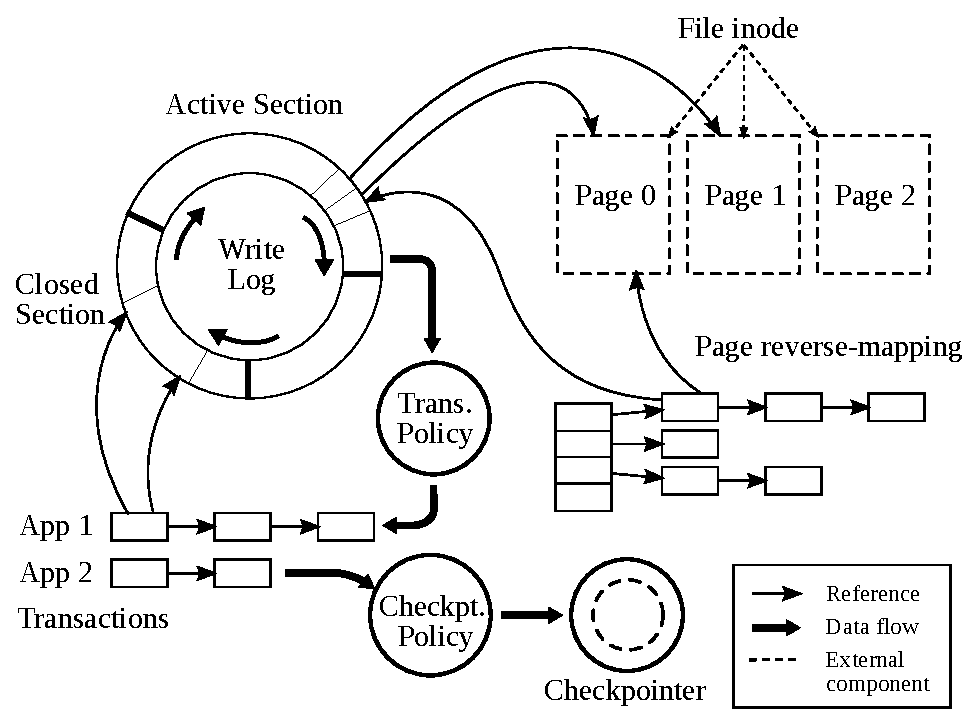
\includegraphics[width=0.8\columnwidth]{arch}
  \caption{MobiFS系统架构图}
  \label{fig:arch}
\end{figure}

MobiFS主要由五个模块构成:(1)页缓存,负责在内存中存储文件数据;(2)写日志,负责维护写操作的历史,由按序排列的许多记录项构成,每个记录项会引用一个页缓存中的物理页;(3)事务,写日志中的若干记录项归并为一组,它们的一致性不受覆写和重排序等优化的影响;(4)检查点生成器(checkpointer),负责调用底层闪存管理组件以原子性方式完成事务的持久化;(5)策略引擎,负责依据优化算法划分事务的边界,监听用户交互行为,并决定生成检查点的事务和时机。图~\ref{fig:arch} 描绘了MobiFS的系统架构。

MobiFS的设计充分考虑了与现有操作系统(Linux)的兼容和组件重用。它与操作系统共享现有的页缓存结构。对于页缓存的每个写操作,都会记入写日志,通常体现为在当前事务中(写日志的末尾)追加一个记录项,除非当前事务已经包含目标页地址的记录项。为此,我们需要维护一组从页地址到写日志项的逆向映射,以判断目标页地址是否已经存在于事务中。基于写日志和逆向映射,MobiFS建立起原子性事务机制。每个事务定义了可以进行覆写和重排序等优化的一个特定范围。最终,策略引擎指导检查点生成器保存事务到闪存,同时不影响用户交互。策略引擎根据每个手机应用甚至是用户的行为及其统计指标,做出动态的智能的判断。

在一个典型的配置中,不同手机应用会拥有自己独立的写日志和事务,但它们共享逆向映射、策略引擎和检查点生成器等组件。

\section{多版本缓冲事务技术}

在写日志中,可能同时引用逻辑上同一个缓冲页的多个物理版本。多版本缓冲事务用来管理这种关系。覆写和重排序等优化手段只允许用于单个多版本缓冲事务内部。由于检查点生成器可保证一个事务整体的持久化和原子性,这些优化不会导致闪存数据的任何不一致状态。

\subsection{写日志}

写日志是应用所有写操作按时间排列的历史记录。写日志包含两个段:活跃段(active section)处在写日志的末尾,新的记录项会被插入活跃段;闭合段(closed section)则包含准备生成检查点的记录项。 
 
在Android平台上,一份写日志的范围涵盖一个手机应用访问的所有目录。手机应用可能使用数据库SQLite保存数据,而SQLite是一个嵌入式数据库,它与每个应用捆绑的相关文件也需要托管给MobiFS,包含在应用的写日志范围内。
 
我们之所以能够面向特定应用进行写优化,一个重要原因在于手机应用的数据路径是静态的和相互隔离的,从而避免了应用间的一致性问题。当然,的确存在多个应用共享文件数据的情况,例如文件浏览器和相册应用可能同时管理照片存放的目录。这种情况下,相关应用需要在程序逻辑层面进行处理。即便不使用MobiFS,在现有Android的文件系统上,应用同样需要处理这类情况(例如,用户通过文件浏览器手动删除了相册中原本可见的照片)。 

\subsection{事务和版本}

一个多版本缓冲事务在其生命周期内经历三个状态:(1)当处于打开状态时,一个事务接收新的记录项,而这些记录项构成写日志中的活跃段。(2)当进入闭合状态时,该事务的所有记录项不再可以更改,转入写日志的闭合段。从打开状态到闭合状态的转换是单向的,不可逆的。(3)当进入提交状态时,该事务所有记录项对应的物理缓存页被检查点生成器原子性地刷出到闪存。成功提交之后,该事务及其记录项即从写日志中消除。 
 
当一个写操作到达时,MobiFS需要处理三种情况:(1)如果要写入的目标页不存在于逆向映射中,那么意味着写操作将进入一个未被写日志涵盖的页。MobiFS会在写日志中追加一个记录项,建立到缓存页的映射,并建立逆向映射。(2)如果逆向映射已经存在且指向一个写日志闭合段中的记录项,那么意味着写操作想要写入一个被保护的只读的事务。为此MobiFS对目标页执行写时拷贝(copy-on-write),并为新的页副本添加写日志记录项及映射/逆向映射。(3)如果逆向映射存在且指向一个写日志活跃段中的记录项(即打开的事务),那么意味着目标页不在被保护的闭合事务中,写操作可以直接更改目标页。

\subsection{故障复原}

多版本缓冲事务的边界不一定要和应用调用fsync()的时间对齐。在系统故障复原时,MobiFS依赖底层闪存管理组件,恢复已提交的事务或者回滚生成不完整检查点的事务。以我们基于日志文件系统Ext4组件的原型系统为例,它或者丢掉不完整的内部日志以回滚到之前的事务,或者重放日志内容恢复状态一致的事务。因此,文件系统或者数据库在系统复原后看到的数据总是对应于历史上某一个瞬间的状态。我们可以看到,MobiFS保证数据的一致性,而不保证严格意义上的已提交事务的持久性。

\subsection{检查点生成}

检查点生成器主要有两个职责。首先,它调用底层闪存管理组件保存事务数据。其次,当MobiFS载入时,检查所有分区并恢复一致的数据或回滚丢弃不一致的数据。很多现有文件系统(如Ext4和Btrfs)的闪存管理组件都可以很容易地进行重用。检查点生成器提供如下四个接口。 

\begin{itemize}
\item BEGIN\_TRANSACTION:在事务提交的开始调用,标志原子性保护的开端。 
\item SUBMIT\_ENTRY:在事务提交开始后,对该事务中每个写日志记录项调用。 
\item END\_TRANSACTION:在提交所有记录项后,即事务提交结束时,进行调用,标志原子性保护的结束。 
\item WAIT\_SYNC:支持非阻塞的调用方式,用于等待数据写入闪存。 
\end{itemize}

底层闪存管理组件需要保证在BEGIN\_TRANSACTION和END\_TRANSACTION调用之间写入的数据具有持久性和原子性。 

\section{优化策略和算法}

有两类策略在策略引擎中运行,事务划分策略和检查点生成策略。前者解决何时关闭一个事务的问题,后者解决何时将闭合事务写入闪存的问题。我们采用的通用规则是在手机处于空闲状态时(例如用户在阅读屏幕上的内容而没有操作行为的时候)生成检查点。我们的策略引擎设计为一个可扩展的框架,故有别于以下算法的其他具体策略亦可以使用。

\subsection{概述}

策略设计需要平衡多个相互冲突的目标:尽量少的数据滞后量,尽量高的能量效率和应用响应度。我们将三者的关系组织为一个可扩展的模块化的策略框架。 

MobiFS的策略框架包含三个模块:(1)事务划分模块,根据$e$曲线决定事务的边界,目标是获得尽量高的能量效率(\ref{subsec:point}节);该策略不依赖于有关用户操作分布的不现实的假设。(2)用户行为动态预测模块,根据预测结果可以推迟事务生成检查点的时间,目标是尽量不影响应用的响应度(\ref{subsec:interval}节)。(3)调度模块,协调多个应用的检查点生成过程(\ref{subsec:sched}节)。 
 
我们将能耗优化和响应度优化的策略独立分开,以避免复杂却又基于简化假设的多目标优化算法。我们的方式使得算法实现简洁而对实际系统有效。这里使用的很多技巧来源于我们大量第一手的优化经验。 

\subsection{事务划分算法}
\label{subsec:point}

\begin{figure}
\centering
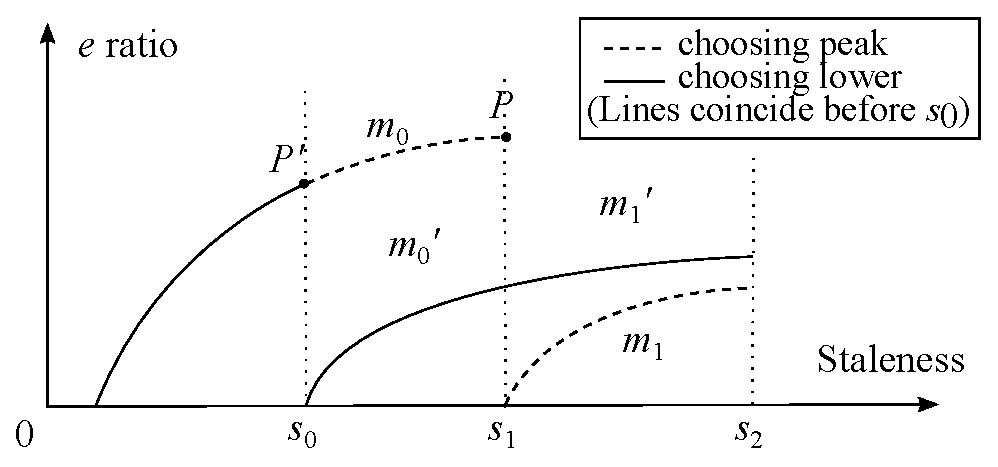
\includegraphics[width=0.7\columnwidth]{figures/tpl}
\caption{由选择不同的事务结束点产生的不同$e$曲线}
\label{fig:tpl}
\end{figure}

增加数据滞后量可以增加数据覆写的概率,从而节约数据冲刷量和相应的能耗,但付出的代价是更高的数据丢失的风险。所以我们面临这样的问题:MobiFS应该在多大程度上为减少能耗而增加数据滞后量?传统工作~\cite{Ma:2011:LPF:1989323.1989325, Mickens:2014:BFC:2616448.2616473, Ports:2010:TCA:1924943.1924963}仅通过设置一个较大的滞后量阈值来决定,而我们采用量化的动态的策略,依照每数据滞后量单元所节约的能耗量,即$e$比率(\ref{subsec:insight}节)来决定。直观来看,$e$曲线的顶点是最佳折衷点,因为对应的能耗节约率最高。我们的设计原则是减少数据丢失风险,除非有特定的原因不这样做(为提升能量效率等)。 

具体地,我们提出最佳折衷点定位算法(tradeoff point location,TPL),用于确定写日志中结束当前事务的记录项。每个来自应用的写操作都会增加数据滞后量,对应于$e$曲线上的一个点。当一个事务关闭时,$e$曲线重新从$e=0$开始计算,如图\ref{fig:tpl}所示。最理想地,结束事务的最佳点应当在$e$值最高的曲线顶点。我们采用反证法,假设另一个算法决定在$P'$点关闭当前事务,此时$x = s_0$,而曲线顶点$P$处于不同的位置$x = s_1$。那么我们可以在保持下一个事务结束点$x = s_2$不变的前提下,通过将当前事务结束点变为$P$来获得更多的能耗节约量。将当前事务结束点由$P'$变为$P$可以提高数据覆写发生的概率\footnote{注意这不是一个严格的数学证明。虽然可以构造出反例,但总体来说可能性更大。}。不失一般性,我们令$s_0 < s_1$;在$[s_0, s_1]$($[s_1, s_2]$)区段,我们算法的覆写数据量为$m_0$($m_1$),假设的算法的覆写数据量是$m_0'$($m_1'$)。那么我们有$m_0 - m_0' > m_1' -
m_1$,原因如下:区段$[s_0, s_1]$上,$e$曲线仍然在快速上升,表明可以覆写的数据量较大,但却被假设算法截断,会导致大量可以覆写的数据丧失覆写机会;相反地,由于$P$是曲线顶点,如果不被截断,曲线在$[s_1, s_2]$区段上是下降的,意味着较少的数据可以被覆写。上述公式简单等价变换可得$m_0 + m_1 > m_0' + m_1'$。综上,在$P$点截断曲线是限制数据滞后量的一种手段,而采用我们的策略可以尽可能多地增加数据覆写的可能。
 
在实际中,我们还需要应对其他一些挑战。曲线会出现波动导致算法定位在局部最优解,为此我们使用一个滑动窗口进行线性拟合来屏蔽这些波动。具体地,算法记录$e$曲线上过去$k$个点,拟合出一条曲线,然后根据其斜率判断是否到达顶点。我们之所以选择线性拟合,而不是更高阶的曲线拟合,是因为策略引擎对于每次写操作都要进行计算,算法复杂度会影响CPU的能耗。与此同时,我们设置了一个数据滞后量(或者冲刷间隔时间)的上限,以防止为等待顶点出现而无穷等待的情况。该算法的评测参见\ref{subsec:energy}节。

\subsection{行为间隔预测}
\label{subsec:interval}

\subsection{事务调度}
\label{subsec:sched}

\section{系统实现和效能评测}

\subsection{系统实现}

\subsection{评测方法}

\subsection{内存占用评测}

\subsection{应用和用户感知评测}

\subsection{应用响应度评测}

\subsection{能耗评测}
\label{subsec:energy}

\section{本章小结}


\chapter{小缓冲器组技术及事务内存性能优化}
\label{chap:sba}

\section{基于非易失性内存的缓冲器管理}

\section{小缓冲器组技术}

\section{快照隔离及只读事务性能优化}

\section{系统实现和性能评测}

\section{本章小结}


\chapter{双模式检查点生成技术及混合内存性能优化}
\label{chap:thnvm}

\section{软件透明的一致性保证机制}

新兴的字节编址的(byte-addressable)非易失性内存介质,诸如STT-RAM~\cite{4443191}、PCM~\cite{Raoux:2008:PRA}和ReRAM~\cite{5607274}等预示着持久化内存系统,一个在内存和存储栈上的新的中间层。持久化内存系统融合了传统内存系统(快速的load/store指令接口)和存储系统(数据持久化)的优良特性,模糊了两者之间的界限。它给应用带来的一个重要的益处是,可以通过load/store指令高效地直接地访问内存中的持久化数据,而不需要与存储设备进出换页、在(反)序列化时更改数据格式以及触发臃肿的系统调用。

持久化内存相对于传统的易失性内存系统引入了一个关键的要求,系统故障时的一致性保证~\cite{Lamb:1991:ODS,Copeland:1989:CSR,Shapiro:1999:EFC}。这要求持久化内存系统,在掉电或系统失效等故障出现时,依然能够保证数据的一致性不受部分或是乱序的NVM写的影响。我们以原子性地更新保存在NVM上的数据结构A和B为例,总会有对A或B的一个更改会先于其他写入NVM。如果系统在一个更改完成之后出现故障或掉电,两个数据结构可能处于不一致的中间状态,只包含部分更改。对于传统易失性内存,这不是一个问题,因为程序恢复后内存中的数据都会丢失。但对于持久化内存,这些不一致的数据会一直保留。所以,持久化内存系统需要保证保存到NVM的数据可以在系统重启后恢复到一个一致的状态,即维持数据的一致性。维持数据的一致性原本仅是对磁盘或闪存等存储系统的要求,但将数据持久化引入内存后,它即成为内存系统同样面临的一个挑战。

大多数之前的持久化内存设计依赖于程序员的人工努力来保证系统故障时的数据一致性。应用的开发人员需要显式地使用特定的编程模型和软件接口来访问和操作内存中的持久化数据。这些软件接口构建于为持久化内存定制的运行时库~\cite{Condit:2009:BIT:1629575.1629589,Volos:2011:MLP:1950365.1950379}或硬件架构~\cite{Zhao:2013:KCP:2540708.2540744}。这种设计似乎给程序员提供了对数据持久化的完全控制,但要求程序员管理持久化内存会带来至少三方面不良影响。首先,应用开发者必须用新的编程接口API来实现程序或者深度更改遗留代码,通常要显式地声明和划分持久的和临时数据结构。其次,大多数之前的持久化内存设计需要使用事务性内存控制版本和对NVM写的顺序,而事务性内存的扩展性依然面临挑战。第三,现在持久性内存的编程模型可能基于很多种语义和软件接口实现,会带来兼容性和移植性问题。为此,我们工作的目标是设计高效的故障时数据一致性保障机制,使得持久化内存的使用范围得到扩展而不必需要复杂的应用更改。

我们提出了THNVM,一种新的支持对软件透明的故障时数据一致性的持久化内存设计。它允许基于事务的和基于锁的程序直接在持久化内存硬件上运行。THNVM使用DRAM和NVM混合的架构和高效的硬件辅助的检查点生成技术来达到DRAM水平的性能。这里的一个关键挑战是减少由于生成检查点而导致的应用停滞时间。我们发现,在停滞时间和元数据存储开销之间存在一个折衷。在较小的粒度上生成检查点,带来的停滞时间可以比较短,而对应元数据占用的空间却会非常大;在较大的粒度上生成检查点,可以降低元数据占用的空间,但是会导致较长的停滞时间。因此,单一的检查点生成技术(或者基于小粒度或者基于大粒度)难以达到最优的效果。为了解决这一问题,我们提出了双模式检查点生成机制,它可以同步地为分散的和集中的内存写分别基于CPU缓存块粒度和操作系统页粒度生成检查点。与先前使用写时拷贝(copy-on-write,COW)或日志技术的持久化内存设计相比,THNVM显著减小了存储的损耗并增加了内存带宽的利用率。

特别地,本章工作做出了如下几点贡献:(1)我们提出了一种新的持久化内存设计,支持对软件透明的故障时数据一致性保障。我们的设计允许基于事务的和基于锁的应用通过load/store指令接口使用持久化内存。(2)对于生成检查点的粒度,我们定位了程序停滞时间和元数据空间占用之间的权衡关系。在任意一个粒度上追踪对持久化内存的更改都不是最优的。(3)我们设计了一个新的双模式检查点生成技术。我们的技术比页粒度的检查点生成机制减少了86.2\%的停滞时间,而仅比缓存块粒度的检查点生成机制多用26\%的内存控制器硬件空间。(4)我们在内存模拟器上实现了双模式检查点生成机制,使用我们经过形式化证明的一致性协议。它可以在保证数据一致性的同时,将检查点生成过程和程序执行重叠。我们的解决方案可以达到不提供一致性支持的全DRAM系统性能的95.1\%。

\section{现有技术缺陷}

THNVM的设计有三个本质特性:软件透明,检查点生成,以及双模式。本节讨论我们开发这三种特性的原因。

\subsection{软件一致性保障技术的缺陷}

\begin{figure}[t]
\centering \includegraphics[width=\columnwidth]{motivation-code}
  \caption{实例代码:向持久化的哈希表中插入一个项。分别采用(a)传统的软件接口或(b)软件透明的THNVM。}
\label{fig:motivation-code}
\end{figure}

之前大多数持久化内存设计~\cite{Condit:2009:BIT:1629575.1629589,Volos:2011:MLP:1950365.1950379,Coburn:2011:NMP:1950365.1950380,Zhao:2013:KCP:2540708.2540744,Venkataraman:2011:CDD:1960475.1960480}要求应用开发者显式地定义持久性数据并使用特定库来访问数据——故障时数据一致性保障机制与软件的语义紧耦合。我们通过图\ref{fig:motivation-code}中的实例代码来展示这种持久化内存设计的不足。该图比较了一个更新持久性哈希表项的软件方法的两种实现(代码改编自STAMP~\cite{Cao:2008:STA})。图\ref{fig:motivation-code}(a)展示了使用类似于现有设计~\cite{Condit:2009:BIT:1629575.1629589, Volos:2011:MLP:1950365.1950379}的软件事务的实现;而图\ref{fig:motivation-code}(b)中的实例代码采用了THNVM的软件透明的故障时数据一致性支持。我们可以看到,在支持数据一致性时涉及软件支持,会有多方面的不足。

首先,划分临时性和持久性数据很麻烦而且容易出错。图\ref{fig:motivation-code}(a)展示了许多无法避免的标记。程序员需要对软件行为有深入的了解,并且小心地确定哪些数据结构需要持久化以及如何操控这些数据。例如,图\ref{fig:motivation-code}(a)的第3行仅当这个哈希表实现固定数目的桶时才是正确的。

其次,在一个统一的地址空间内,临时性和持久性数据之间的引用需要小心的管理。然而,对该问题的基于软件的解决方案并非最佳。例如,为了处理NV-to-V指针(非易失性指针指向易失性数据,图\ref{fig:motivation-code}(a)的第8行),NV-heaps~\cite{Coburn:2011:NMP:1950365.1950380}会简单地抛出一个运行时错误以禁用此类指针。

第三,应用需要使用事务,通常是通过事务性内存接口(例如被Mnemosyne~\cite{Volos:2011:MLP:1950365.1950379}使用的TinySTM~\cite{Felber:2008:DPT}),来更新持久化数据,如图\ref{fig:motivation-code}(a)所示。遗憾的是,事务性内存,不论基于硬件还是基于软件,存在多方面的可扩展性问题~\cite{Cascaval:2008:STM:1454456.1454466,Pankratius:2011:STM:1989493.1989500,Dice:2009:EEC:1508244.1508263}。此外,开发人员必须使用新的API来实现或者重写各种代码库和程序,需要不可忽略的人工投入。不熟悉这些新API的程序员需要一个痛苦的学习过程。

最后,应用需要构建在特定的库之上,例如libmnemosyne~\cite{Volos:2011:MLP:1950365.1950379}和
NV-heaps~\cite{Coburn:2011:NMP:1950365.1950380}。这会很大程度上降低持久化内存应用的移植性——在一个库上实现的应用,如果想采用其他的库,需要重新实现。编译器确实可以在一定程度上减轻程序员实现和移植代码的负担。然而,编译器会无差别地插装所有内存的读和写操作,带来可见的性能损耗。我们在GCC libitm~\cite{libitm}上实验了STAMP事务性基准测试~\cite{Cao:2008:STA},结果插装本身最多可带来高达8\%的性能损失。

我们采用了允许软件程序直接访问持久化内存的使用模型。如图\ref{fig:motivation-code}(b)所示,我们可以不更改代码而实现数据结构的持久化。

\subsection{日志及写时拷贝技术的缺陷}



\subsection{粒度的权衡}

\section{双模式检查点生成技术}

\subsection{系统定义}

\subsection{基于块重映射的检查点生成}

\subsection{基于页回写的检查点生成}

\subsection{双重检查点生成机制}

\section{一致性机制的状态机表达}

\section{一致性机制的正确性证明}

\section{系统实现}

\subsection{地址空间管理}

\subsection{元数据管理}

\subsection{数据保存}

\subsection{数据恢复}

\section{系统测评}

\subsection{实验设置}

\subsection{微基准测试}

\subsection{存储类基准测试}

\subsection{计算类基准测试}

\subsection{敏感度分析}

\section{本章小结}


\chapter{双模式检查点生成技术}
\label{chap:thynvm}

新兴的字节编址的(byte-addressable)非易失性内存介质,诸如STT-RAM~\cite{4443191}、PCM~\cite{Raoux:2008:PRA}和ReRAM~\cite{5607274}等预示着持久化内存系统,一个在内存和存储栈上的新的中间层。持久化内存系统融合了传统内存系统(快速的load/store指令接口)和存储系统(数据持久化)的优良特性,模糊了两者之间的界限。它给应用带来的一个重要的益处是,可以通过load/store指令高效地直接地访问内存中的持久化数据,而不需要与存储设备进出换页、在(反)序列化时更改数据格式以及触发臃肿的系统调用。

持久化内存相对于传统的易失性内存系统引入了一个关键的要求,系统故障时的一致性保证~\cite{Lamb:1991:ODS,Copeland:1989:CSR,Shapiro:1999:EFC:319151.319163}。这要求持久化内存系统,在掉电或系统失效等故障出现时,依然能够保证数据的一致性不受部分或是乱序的NVM写的影响。我们以原子性地更新保存在NVM上的数据结构A和B为例,总会有对A或B的一个更改会先于其他写入NVM。如果系统在一个更改完成之后出现故障或掉电,两个数据结构可能处于不一致的中间状态,只包含部分更改。对于传统易失性内存,这不是一个问题,因为程序恢复后内存中的数据都会丢失。但对于持久化内存,这些不一致的数据会一直保留。所以,持久化内存系统需要保证保存到NVM的数据可以在系统重启后恢复到一个一致的状态,即维持数据的一致性。维持数据的一致性原本仅是对磁盘或闪存等存储系统的要求,但将数据持久化引入内存后,它即成为内存系统同样面临的一个挑战。

大多数之前的持久化内存设计依赖于程序员的人工努力来保证系统故障时的数据一致性。应用的开发人员需要显式地使用特定的编程模型和软件接口来访问和操作内存中的持久化数据。这些软件接口构建于为持久化内存定制的运行时库~\cite{Condit:2009:BIT:1629575.1629589,Volos:2011:MLP:1950365.1950379}或硬件架构~\cite{Zhao:2013:KCP:2540708.2540744}。这种设计似乎给程序员提供了对数据持久化的完全控制,但要求程序员管理持久化内存会带来至少三方面不良影响。首先,应用开发者必须用新的编程接口API来实现程序或者深度更改遗留代码,通常要显式地声明和划分持久的和临时数据结构。其次,大多数之前的持久化内存设计需要使用事务性内存控制版本和对NVM写的顺序,而事务性内存的扩展性依然面临挑战。第三,现在持久性内存的编程模型可能基于很多种语义和软件接口实现,会带来兼容性和移植性问题。为此,我们工作的目标是设计高效的故障时数据一致性保障机制,使得持久化内存的使用范围得到扩展而不必需要复杂的应用更改。

我们提出了ThyNVM,一种新的支持对软件透明的故障时数据一致性的持久化内存设计。它允许基于事务的和基于锁的程序直接在持久化内存硬件上运行。ThyNVM使用DRAM和NVM混合的架构和高效的硬件辅助的检查点生成技术来达到DRAM水平的性能。这里的一个关键挑战是减少由于生成检查点而导致的应用停滞时间。我们发现,在停滞时间和元数据存储开销之间存在一个折衷。在较小的粒度上生成检查点,带来的停滞时间可以比较短,而对应元数据占用的空间却会非常大;在较大的粒度上生成检查点,可以降低元数据占用的空间,但是会导致较长的停滞时间。因此,单一的检查点生成技术(或者基于小粒度或者基于大粒度)难以达到最优的效果。为了解决这一问题,我们提出了双模式检查点生成机制,它可以同步地为分散的和集中的内存写分别基于CPU缓存块粒度和操作系统页粒度生成检查点。与先前使用写时拷贝(copy-on-write,COW)或日志技术的持久化内存设计相比,ThyNVM显著减小了存储的损耗并增加了内存带宽的利用率。

特别地,本章工作做出了如下几点贡献:(1)我们提出了一种新的持久化内存设计,支持对软件透明的故障时数据一致性保障。我们的设计允许基于事务的和基于锁的应用通过load/store指令接口使用持久化内存。(2)对于生成检查点的粒度,我们定位了程序停滞时间和元数据空间占用之间的权衡关系。在任意一个粒度上追踪对持久化内存的更改都不是最优的。(3)我们设计了一个新的双模式检查点生成技术。我们的技术比页粒度的检查点生成机制减少了86.2\%的停滞时间,而仅比缓存块粒度的检查点生成机制多用26\%的内存控制器硬件空间。(4)我们在内存模拟器上实现了双模式检查点生成机制,使用我们经过形式化证明的一致性协议。它可以在保证数据一致性的同时,将检查点生成过程和程序执行重叠。我们的解决方案可以达到不提供一致性支持的全DRAM系统性能的95.1\%。

\section{软件透明的一致性保证机制}

ThyNVM的设计有两个本质特性,软件透明和检查点生成。本节讨论我们开发这两个特性的原因。

\subsection{软件一致性保障技术的缺陷}

\begin{figure}[!h]
\centering \includegraphics[width=0.9\linewidth]{motivation-code}
  \caption{实例代码:向持久化的哈希表中插入一个项。分别采用(a)传统的软件接口或(b)软件透明的ThyNVM。}
\label{fig:motivation-code}
\end{figure}

之前大多数持久化内存设计~\cite{Condit:2009:BIT:1629575.1629589,Volos:2011:MLP:1950365.1950379,Coburn:2011:NMP:1950365.1950380,Zhao:2013:KCP:2540708.2540744,Venkataraman:2011:CDD:1960475.1960480}要求应用开发者显式地定义持久性数据并使用特定库来访问数据——故障时数据一致性保障机制与软件的语义紧耦合。我们通过图\ref{fig:motivation-code}中的实例代码来展示这种持久化内存设计的不足。该图比较了一个更新持久性哈希表项的软件方法的两种实现(代码改编自STAMP~\cite{Cao:2008:STA})。图\ref{fig:motivation-code}(a)展示了使用类似于现有设计~\cite{Condit:2009:BIT:1629575.1629589, Volos:2011:MLP:1950365.1950379}的软件事务的实现;而图\ref{fig:motivation-code}(b)中的实例代码采用了ThyNVM的软件透明的故障时数据一致性支持。我们可以看到,在支持数据一致性时涉及软件支持,会有多方面的不足。

首先,划分临时性和持久性数据很麻烦而且容易出错。图\ref{fig:motivation-code}(a)展示了许多无法避免的标记。程序员需要对软件行为有深入的了解,并且小心地确定哪些数据结构需要持久化以及如何操控这些数据。例如,图\ref{fig:motivation-code}(a)的第3行仅当这个哈希表实现固定数目的桶时才是正确的。

其次,在一个统一的地址空间内,临时性和持久性数据之间的引用需要小心的管理。然而,对该问题的基于软件的解决方案并非最佳。例如,为了处理NV-to-V指针(非易失性指针指向易失性数据,图\ref{fig:motivation-code}(a)的第8行),NV-heaps~\cite{Coburn:2011:NMP:1950365.1950380}会简单地抛出一个运行时错误以禁用此类指针。

第三,应用需要使用事务,通常是通过事务性内存接口(例如被Mnemosyne~\cite{Volos:2011:MLP:1950365.1950379}使用的TinySTM~\cite{Felber:2008:DPT}),来更新持久化数据,如图\ref{fig:motivation-code}(a)所示。遗憾的是,事务性内存,不论基于硬件还是基于软件,存在多方面的可扩展性问题~\cite{Cascaval:2008:STM:1454456.1454466,Pankratius:2011:STM:1989493.1989500,Dice:2009:EEC:1508244.1508263}。此外,开发人员必须使用新的API来实现或者重写各种代码库和程序,需要不可忽略的人工投入。不熟悉这些新API的程序员需要一个痛苦的学习过程。

最后,应用需要构建在特定的库之上,例如libmnemosyne~\cite{Volos:2011:MLP:1950365.1950379}和
NV-heaps~\cite{Coburn:2011:NMP:1950365.1950380}。这会很大程度上降低持久化内存应用的移植性——在一个库上实现的应用,如果想采用其他的库,需要重新实现。编译器确实可以在一定程度上减轻程序员实现和移植代码的负担。然而,编译器会无差别地插装所有内存的读和写操作,带来可见的性能损耗。我们在GCC libitm~\cite{libitm}上实验了STAMP事务性标准测试~\cite{Cao:2008:STA},结果插装本身最多可带来高达8\%的性能损失。

我们采用了允许软件程序直接访问持久化内存的使用模型。如图\ref{fig:motivation-code}(b)所示,我们可以不更改代码而实现数据结构的持久化。

\subsection{日志及写时拷贝技术的缺陷}

前人基于软件的持久化内存设计,大部分通过修改现有软件事务性内存库、文件系统或者数据库实现,采用日志~\cite{Volos:2011:MLP:1950365.1950379, Coburn:2011:NMP:1950365.1950380}或者写时拷贝技术~\cite{Condit:2009:BIT:1629575.1629589,
Venkataraman:2011:CDD:1960475.1960480}维持数据一致性。然而,两种技术为支持数据一致性保障会引入较大的性能损耗。

日志可能消耗比原始数据大很多的NVM空间,因为每个日志项都是一个既包含数据又包含元数据(例如数据所在的地址)的元组,而且通常每次写操作都需要记录~\cite{Volos:2011:MLP:1950365.1950379,
Coburn:2011:NMP:1950365.1950380}\footnote{某些对于日志的改进或变形~\cite{1003568}使用一个索引结构来合并更新。该设计即与我们双模式之一类似。}。此外,日志重放增加了故障后系统恢复时间,会抵消使用NVM而不是顺序访问的块设备带来的快速数据恢复的好处。

写时数据拷贝有两个缺点。首先,拷贝操作代价较大,会引发较长的停滞时间。其次,它不可避免地会复制未更改的数据,消耗额外的NVM带宽。这个缺陷在更新的地址很分散时尤为突出。

相比之下,生成检查点是一种更加灵活的方法,它定期地将易失性的数据及元数据写入NVM形成一致的内存数据的快照。我们仔细挑选和协调两种检查点生成模式,使它们同步地在不同粒度上工作,从而避免日志和写时拷贝的弊端。


\section{双模式检查点生成技术}

\subsection{粒度的权衡}

CPU缓存在块粒度上(典型配置为64字节)管理数据;操作系统在页粒度上(典型配置为4KB)管理数据。我们发现两个不同的粒度会带来一个在检查点生成停滞时间和元数据存储空间之间的折衷。

当我们选择在缓存块粒度上追踪持久化内存的更改时,各个细粒度写如果直接发送到NVM,可以在一两次总线传输的延迟内完成。这样,ThyNVM只需要在生成检查点时将追踪这些数据所用的元数据进行持久化即可。这些元数据可以保存在一个表中,每个表项保存一个从缓存块在内存中的地址到它实际检查点或工作数据位置的映射。这种模式的缺点在于元数据表项的数量是按页粒度追踪数据所需表项的64倍,因为每个页包含64个缓存块。相反地,如果我们在页粒度上追踪持久化内存的更改,我们可以极大地降低保存元数据表所需的硬件空间开销。然而把整页的数据写入NVM所造成的延迟,远大于更新一个缓存块。为了提升系统性能,ThyNVM使用DRAM来缓冲页粒度的更新,一段时间后再在NVM上生成这些页的检查点。尽管如此,将整页数据从DRAM传送到NVM依然会给系统带来较长的停滞时间。

考虑到如上的折衷,只在一个粒度上追踪持久化内存的更改不是最佳方案。这种情况下,我们需要开发一种双粒度的检查点生成技术。

\begin{figure}[!h]
\centering
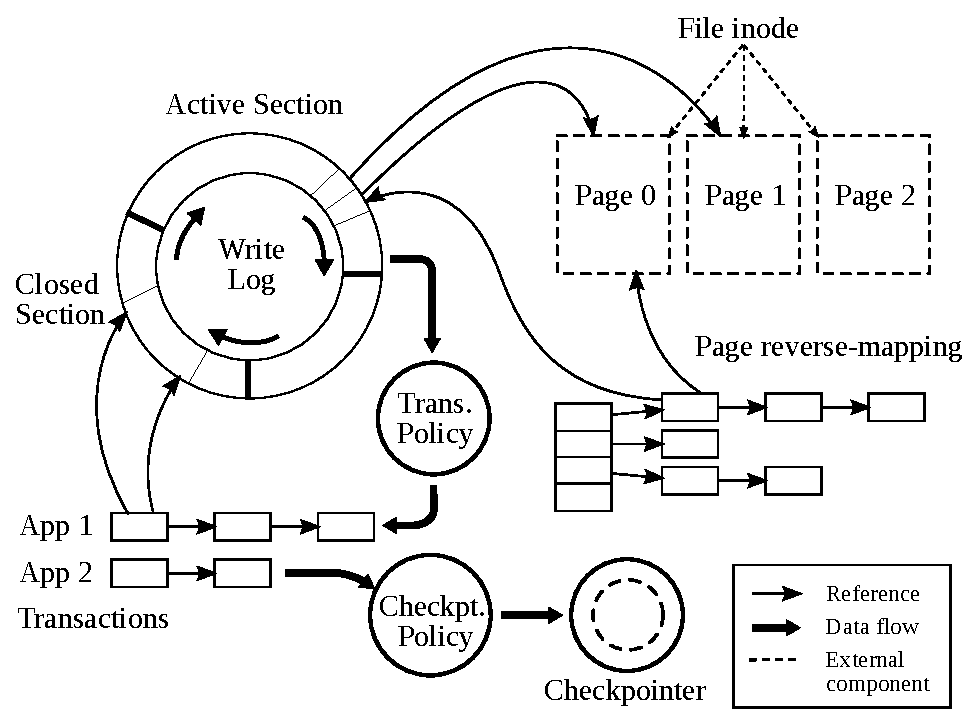
\includegraphics[width=0.9\linewidth]{arch}
\caption{ThyNVM的总体架构图。}
\label{fig-arch}
\end{figure}

ThyNVM采用DRAM和NVM的混合架构,基于硬件实现,提供软件透明的故障时数据一致性保障。ThyNVM以透明于应用程序的方式保障所有内存数据在故障时的一致性。为了利用在不同粒度持久化数据带来的不同特性,我们提出了一种新的双模式检查点生成机制。它可以同时在两个粒度上生成内存数据的检查点:分散的写在缓存块粒度上生成检查点,使用块重映射模式(第\ref{subsec:block-remap}节);集中的写在页粒度上生成检查点,使用页回写模式(第\ref{subsec:page-writeback}节)。

另外,我们提出了两种机制来协调双模式检查点生成(第\ref{subsec:coordination}节)。第一,我们允许相对较快的块重映射模式来暂时接管原本应该由较慢的页回写模式处理的写。这样做可以显著减少检查点生成阻塞程序执行的时间。第二,我们定期地依据程序执行时访问内存的特点在两种模式之间迁移数据页。这样做可以有效保证检查点生成模式和其处理的写的行为相匹配。

图\ref{fig-arch}绘制了ThyNVM架构总览。DRAM和NVM部署在内存总线上,并映射到同一个物理内存地址空间中。该地址空间暴露给操作系统。我们更改了内存控制器,增加了一个检查点生成控制器,和两个用于维护内存访问元数据的地址转换表。这两个表分别是在缓存块粒度和页粒度管理元数据的块转换表(block translation table,BTT)和页转换表(page translation table,PTT)。

\subsection{系统定义}

\textbf{失效模型}:ThyNVM允许软件应用在诸如系统死机、掉电等故障发生后,从一个一致的内存数据检查点开始,继续CPU执行。为此,我们需要定期将内存中的数据的更新和CPU状态生成检查点,这其中包括CPU寄存器、写缓冲、脏缓存块以及内存控制器的写队列。我们的检查点生成机制保护内存数据和CPU状态的一致性不因系统故障而被污染。

\begin{figure}[!h]
\centering
\includegraphics[width=0.9\linewidth]{epoch-before}\\
{\small (a) 采用检查点生成时暂停全系统的时间单元模型}
\includegraphics[width=0.9\linewidth]{epoch-after}\\
{\small (b) ThyNVM采用的时间单元模型,可将检查点生成和程序执行相互重叠。该模型维护三个版本的数据:活跃的工作数据($W_{active}$)、最近检查点数据($C_{last}$),和次近检查点数据($C_{penult}$)。\hfill}
\caption{检查点生成系统的时间单元模型。}
\label{fig-epoch}
\end{figure}

\textbf{时间单元模型}:我们逻辑上把程序的执行时间分成连续的时间区段,称为时间单元(epoch,如图\ref{fig-epoch})。每个时间单元包括一个执行阶段和一个检查点生成阶段。执行阶段更新工作数据,而检查点生成阶段持久化内存中的数据和CPU状态。

让执行阶段和检查点生成阶段顺次交替(如图\ref{fig-epoch}(a)所示)会导致显著的性能下降。对于内存访问频繁的负载,检查点生成可以消耗高达35.4\%的程序运行时间。所以,ThyNVM采用了一种将检查点生成阶段和程序执行阶段重叠的时间单元模型~\cite{1003568},以降低该性能损失。我们定义三个连续的时间单元依次为活跃的、最近的和次近的时间单元。如图\ref{fig-epoch}(b)所示,一个新的活跃时间单元(时间单元2)可以在最近时间单元(时间单元1)的执行阶段和次近时间单元(时间单元0)的检查点生成阶段两者中更晚结束的一个之后即开始。

\textbf{数据版本}:执行阶段和检查点生成阶段重合允许两个相邻的时间单元同时访问相同的数据。这对数据一致性的维护带来了两个挑战。第一,相互重合的执行阶段和检查点生成阶段可能会覆盖对方的数据更改,所以我们需要隔离不同时间单元的数据更改;第二,系统失效发生时,活跃时间单元和最近时间单元的数据可能被同时损坏。为了应对这些挑战,ThyNVM维护了连续时间单元下数据的三个版本:\emph{活跃的工作副本 $W_{active}$}、\emph{最近检查点$C_{last}$}和\emph{次近检查点$C_{penult}$} ($C_{last}$和$C_{penult}$既包括内存数据也包括CPU状态)。如图\ref{fig-epoch}(b)所示,当我们在执行时间单元2(更新$W_{active}$)的时候,ThyNVM会同时保留时间单元0的检查点($C_{penult}$)和时间单元1的检查点($C_{last}$);ThyNVM只有在时间单元1的生成检查点阶段结束后,才丢弃时间单元0产生的检查点。一个发生在时间$t$的系统故障,可能损坏时间单元2的工作数据副本以及时间单元1的检查点;此种状况下,我们可以依靠$C_{penult}$回滚到时间单元0。

\subsection{基于块重映射的检查点生成}
\label{subsec:block-remap}

ThyNVM对空间局部性低的数据更新使用块重映射模式进行管理。在每个时间单元的执行阶段,块重映射模式直接将工作数据写入NVM。因此,在相应的检查点生成阶段,ThyNVM可以简单地通过生成元数据(即BTT中的项)的检查点,将工作数据直接转为检查点数据。这样的方法可以大幅减少检查点生成的延迟。

为防止NVM中的更新损坏先前版本的数据,ThyNVM将新的缓存块的更改映射到一个其他的地址。ThyNVM将这类从原始地址到新地址的映射记录在BTT中。随后的内存读操作可以通过查找BTT来确定工作数据副本的有效位置。随后的以原始地址为目标的写操作,只要在同一个活跃时间单元内,可以进行归并,更新到该新地址。在下一个时间单元,该新地址的数据版本自然变为最近的检查点的一部分。NVM保存所有这些检查点数据;并且,ThyNVM在生成检查点阶段的开始会将BTT持久化到NVM。

\subsection{基于页回写的检查点生成}
\label{subsec:page-writeback}

页回写模式用于在页粒度上生成空间局部性较高的写操作的检查点。ThyNVM使用DRAM作为工作数据副本的缓冲。它首先在DRAM上归并内存的更新,然后在每个时间单元结束时生成检查点,将所有DRAM的脏页回写到NVM上。

这里的DRAM在两方面不同于CPU回写缓存或者简单的数据缓冲。第一,内存访问不会触发任何页置换或剔除;脏页只有在生成检查点时被回写。第二,当ThyNVM从DRAM回写一个脏页到NVM时,不可以直接覆盖NVM上原有的检查点数据。所以ThyNVM需要将每个脏页重定向到一个不同的地址上。ThyNVM使用PTT来为内存中的数据页追踪这些地址映射。在检查点生成结束的时候,PTT会被自动持久化到NVM上。这个标志着一个时间单元的结束。

\subsection{协调两种模式}
\label{subsec:coordination}

我们设计了两种机制来协调双模式,以达到如下两个目标:(1)减少程序执行时由于生成检查点带来的停滞时间;(2)调整检查点生成模式来适应动态变化的内存访问行为。

\textbf{两种模式的合作}:块重映射模式允许系统在检查点生成阶段仅持久化元数据。所以,它在检查点生成阶段能够比页回写模式更快地完成。这种情况下,页回写的检查点生成可能阻塞整个程序的执行,因为后续时间单元无法更改还未被写入NVM的DRAM页。为了缓解该问题,ThyNVM通过主动地借用块重映射模式来临时处理那些本该由页回写模式管理的新到的写请求,允许系统开启执行下一个时间单元。通过这种方式,我们隐藏了页回写检查点生成的阻塞时间,实现并行地写NVM和DRAM,并且提高了内存带宽的利用率。

\textbf{两种模式间数据迁移}:ThyNVM需要确保检查点生成采用的模式与数据不断变化的空间局部性和密集度特性相匹配。内存控制器在每个时间单元开始的时候,依据页上近期更改所呈现的空间局部性,决定一些页是否需要从一个模式切换到另一个模式。切换检查点生成模式涉及元数据更新和数据迁移。从页回写模式切换到块重映射模式,我们需要剔除PTT中的相应的项,同时将DRAM中页的可见工作数据移动到NVM上由块重映射模式管理的区域。这样,下次该页的任意缓存块被更改时,内存控制器就会自动将元数据信息添加至BTT中。从块重映射模式切换到页回写模式,我们需要在PTT加入一个项来存储页的元数据,同时将该页所有缓存块数据集中拷贝至DRAM中的相应位置。

\section{系统实现}
\label{sec:implementation}

本节描述内存地址空间管理和ThyNVM引入的硬件更改。我们也给出了ThyNVM操作读、写和检查点的实例,以及恢复由ThyNVM维护的数据的步骤。

\subsection{地址空间管理}
\label{subsec:thnvm-space}

ThyNVM地址空间管理的目标包括(1)在不同的内存位置存放数据的多个版本,以及(2)提供一个有效的一致的数据版本给操作系统。

\textbf{DRAM和NVM中的数据区域:}为了实现第一个目标,我们在DRAM和NVM中维护三个数据区域,每个保存一个数据版本:$W_{active}$、$C_{last}$或者 $C_{penult}$。如图\ref{fig-addr-space}所示,这些区域包括一个DRAM中的工作数据区和两个NVM中的检查点数据区。该工作数据区主要保存由页回写模式管理的活跃工作数据$W^{page}_{active}$,同时在上一个时间单元仍在生成检查点$C_{last}$时,用于缓冲由块重映射模式管理的活跃数据副本$W^{block}_{active}$。检查点区域A和B以交错的方式保存检查点数据$C_{last}$和$C_{penult}$:如果$C_{last}$保存在检查点区域A,我们就把$C_{penult}$写入检查点区域B;反之亦然。另外,如果上一个时间单元已经完成检查点生成,我们以与$C_{last}$交错的方式直接将$W^{block}_{active}$写入检查点区域(即用$W^{block}_{active}$覆写$C_{penult}$如果全内存$C_{last}$已经完整生成)。内存数据的大部分在三个连续时间单元(活跃、上一个和倒数第二个)都不会被更改,这些数据会位于检查点区域B,所以该区域也被称作家区域。另外,我们在检查点区域A开辟专门的内存区域来保存CPU寄存器的检查点。 

\begin{figure}[!h]
\centering
\includegraphics[width=0.9\linewidth]{addr-space}
\caption{ThyNVM的地址空间布局}
\label{fig-addr-space}
\end{figure}

\textbf{物理地址空间到硬件地址空间的映射}。为了实现第二个目标,ThyNVM创建两个地址空间之间的映射关系。硬件地址空间由内存控制器管理,是DRAM和NVM实际的设备地址空间,仅对内存控制器可见。物理地址空间由操作系统管理,是对内存控制器对外提供的内存空间的逻辑视图,实际上包含硬件地址空间里数据的一个子集。我们定义\emph{可见数据}为在当前活跃时间单元内被更新的工作副本或者最近的检查点,即: 
\[
\begin{cases}
        W_{active}, & \text{如果}W_{active}\text{存在}\\
        C_{last}, & \text{如果}W_{active}\text{不存在}
\end{cases}
\]
在数据恢复的时候,我们复原如下的可见数据: 
\[
\begin{cases}
        C_{last}, & \text{如果上一个检查点生成完毕}\\
        C_{penult}, & \text{如果上一个检查点未完整保存}
\end{cases}
\]
我们设计物理地址空间的大小等于硬件地址空间中家区域的大小;也就是说,如果一个数据块或页保存在家区域中,那么它的物理地址等于它的硬件地址。任何没有在BTT/PTT中的数据块/页的可见数据都位于家区域中。

\subsection{元数据管理}

保存在BTT和PTT中的元数据为内存控制器提供必需的信息,以完成如下三个目标:(1)将处理器发出的每个内存请求的物理地址转换成硬件地址;(2)将生成检查点的NVM写指向正确的硬件地址;(3)确定何时在两个检查点生成模式之间迁移数据。ThyNVM在两个地址转换表BTT和PTT中维护元数据。连个表都包含四个列(图\ref{fig:metadata}),包含一个物理地址高位的块/页索引(BTT需要42比特,PTT需要36比特)、一个2比特的版本ID、一个2比特的可见内存区域ID、一个1比特的检查点内存区域ID和6比特的表征空间局部性的写计数器。 

\begin{figure}[!h]
\centering
\includegraphics[width=0.9\linewidth]{metadata}
\caption{BTT和PTT表项的各个列。}
\label{fig:metadata}
\end{figure}

为了达到第一个目标,必要的信息包括:(a)一个请求应当指向的内存区域,以及(b)在该内存区域内物理地址到硬件地址的映射。处理器只能够访问可见数据,所以我们用可见内存区域ID确定对应可见数据所处的内存区域。为了获得硬件地址,我们确保每个表项到表首的偏移数等于相应内存区域中块或页与首块或首页的偏移数(不适用于家区域)。所以,我们可以使用表项的偏移计算出块或页在内存区域中的硬件地址。 

为了达到第二个目标,内存控制器使用检查点内存区域ID来确定一个检查点写的目的内存区域。我们采用和上文相同的方法,通过表项的偏移数来确定硬件地址。 

为了达到第三个目标,内存控制器依据BTT和PTT 的写计数来确定数据的空间局部性。BTT/PTT中的每个写计数器记录了上一个时间单元中对相应物理块/页的写操作的数据;内存控制器在每个时间单元开始时读取并重置写计数器。一个时间单元内对同一个物理页较大数量的写操作(超过预定义的阈值)意味着这个页有较高的空间局部性和写强度。为此,我们下一个时间单元即采用页回写机制来操作对该页的写。写计数器的值如果小于预定义的阈值,表明我们下一个时间单元内应采用块重映射机制。我们实验了不同的阈值,发现从块重映射切换到页回写以及相反切换的阈值分别取22和16时最为有效。
 
\textbf{生成BTT和PTT的检查点:}元数据定位最近的一致的检查点,所以需要在系统故障前后保持持久化。在每个检查点生成阶段,我们在NVM的BTT和PTT备份区域生成BTT和PTT表项的检查点。有一个挑战在于原子性地将BTT/PTT写入NVM。我们使用一个表征BTT/PTT检查点生成是否完成的比特位来维护备份操作的原子性。 

\textbf{BTT和PTT的大小:}BTT表项的数目取决于工作集合的写强度,而PTT表项的数目由DRAM的大小决定。如果有些负载要求GB级的DRAM,巨大的PTT存储代价可以通过虚拟化PTT得到缓解,即在DRAM存储PTT而在内存控制器中缓存部分热点表项~\cite{Meza2012, Yoon2010, Burcea2008}。图\ref{fig:sens-att-len}显示了我们对不同表长度下系统性能进行的敏感度测试。另外,当前硬件的发展和创新使得内存控制器可以拥有复杂的功能,例如,HMC~\cite{HMC:2011}的逻辑层,或者HP的The Machine~\cite{TheMachine:2015}的媒介控制器。这些技术让我们的硬件开销变得可行。

\subsection{服务读写请求}

为了服务一个内存读请求,我们用该请求的物理地址在PTT和BTT中查找。如果该物理地址在两张表中都没有,那么对应的可见数据位于NVM的家区域中。为了服务一个内存写请求,如图~\ref{fig:flow}(a)所示,我们首先使用PTT来确定是使用块重映射模式还是页回写模式——我们对所有PTT不包含的请求采用块重映射,不论它是否包含在BTT中。如果两张表中都不包含,说明对应的数据块位于家区域;这种情况下,我们需要在BTT中添加一个表项,记录该请求带来的元数据更新。对于BTT/PTT溢出,即没有表项空或者可以被替换的情况,我们只得生成一个检查点并开始一个新的时间单元。这样,我们可以安全地将那些表明其最新检查点在家区域的表项清除。

\begin{figure}[!h]
\centering
\includegraphics[width=0.9\linewidth]{flow}
\caption{流程图:\textbf{(a)}在某个时间单元的执行阶段服务一个写请求;\textbf{(b)}在该时间单元的检查点生成阶段生成检查点。为了显示(a)中写入的数据和(b)中检查点数据的关联关系,我们用三个背景方格标记出两种检查点生成模式和它们之间的合作:每个背景方格内,在(a)中存储的数据,在生成检查点的时候,会经历(b)中对应的处理过程。}
\label{fig:flow}
\end{figure}

\textbf{检查点生成:}当我们生成内存数据的检查点时,我们确保元数据在数据之后生成检查点。特别的,我们采用如下的生成检查点的顺序:(1)将缓冲在DRAM中的$W^{block}_{active}$写入NVM;(2)在NVM生成BTT的检查点;(3)将DRAM中的$W^{page}_{active}$写入NVM;(4)在NVM生成PTT的检查点。

\textbf{接收初始的数据访问:}初始地,当系统开始执行,两个地址转换表都是空的;所有可见数据均位于NVM的家区域。因为PTT是空的,我们在第一个时间单元内仅采用块重映射来操作数据更新。之后,ThyNVM将空间局部性高的数据迁移到页回写模式。系统第一次进入稳定状态(即在两种检查点生成模式间迁移的页数下降到一个相对小而稳定的数值)所需要的时间依赖于PTT的大小以及负载的内存访问行为。我们观察到,实验中使用的负载(第\ref{sec:thnvm-eval}节)的最坏情况,可能需要几十个时间单元使2048个PTT表项达到这种稳态。

\subsection{数据冲刷}

为了保证检查点的一致性,在每个时间单元的生成检查点阶段,我们需要将处理器中的数据冲刷到NVM。为此,我们在每个检查点生成阶段的起始,将处理器寄存器保存到NVM,并且冲刷写缓冲和脏数据块;我们还需要在每个检查点生成阶段结束时,在NVM写队列中插入一个分界。 
我们采用基于硬件的机制来执行数据冲刷。内存控制器在一个执行阶段结束时,通过我们添加的信号路径通知CPU。在收到通知后,CPU发出一个冲刷指令将所有内存器的值写入一个NVM上的特别区域,并将写缓存及脏缓存块写入内存控制器。注意我们并不使缓存中的脏数据块失效,类似于Intel的CLWB操作,从而后续的时间单元可以继续访问这些脏数据块。

\subsection{数据恢复} 
对于采用ThyNVM维护故障时数据一致性的系统,数据恢复涉及三个步骤使持久化内存回滚到最新的检查点。首先,我们将BTT和PTT重新载入内存控制器,把它们对应于可见数据版本(定义见第\ref{subsec:thnvm-space}节)的备份从NVM拷贝出来。照此,我们恢复了可以用于恢复数据的元数据信息。第二,我们需要恢复页回写模式管理的可见数据。因为这些页的可见数据版本应当被保存在DRAM中,我们需要将NVM中的检查点拷贝到DRAM中。当元数据和数据都恢复完毕后,我们执行最后一步,从NVM的专属空间重新载入CPU寄存器。 

一旦内存数据和处理器状态被恢复,我们即继续CPU的执行。然而,因为我们并不恢复外部设备(如网卡)的状态,恢复的程序很有可能遇到由于丢失这些设备状态而导致的错误。在我们的故障模型中,系统故障事件以设备错误的形式对软件程序可见。我们依赖软件固有的异常或错误处理机制来应对这些设备错误。在第\ref{sec:thnvm-discuss}节有关于外部状态(如网卡中的状态)丢失的讨论。 

\section{系统测评}
\label{sec:thnvm-eval}

\subsection{实验环境}

本节描述我们使用的模拟器、处理器和内存配置,以及标准测试集。我们的实验基于周期精准的模拟器gem5~\cite{Binkert:2011:GS:2024716.2024718}。我们使用gem5的提供详细时间模型的处理器,并扩展原有经典内存模型~\cite{6844484}。表\ref{table:config}列举了我们模拟用处理器和内存的架构配置和主要详细参数。我们的DRAM和NVM都是采用DDR3接口进行模拟。我们模拟了16~MB的DRAM,以及分别2048个BTT和PTT表项。我们更改了gem5的实现来加入在第\ref{sec:implementation}节描述的ThyNVM的各项机制。每个时间单元的长度被限制在10~ms(与论文~\cite{1003567, 1003568}的配置相近),因为用户或系统软件总是希望系统故障时的数据损失最小。 

\begin{table}[!h]
\centering
\caption{系统配置及参数~\cite{Lee:2009:APC:1555754.1555758}。}
\label{table:config}
\begin{tabular}{l|l}
\toprule[1.5pt]
处理器 & $3~GHz$,按序执行 \\
\hline
L1指令/数据缓存 & 私有$32~KB$,$8$路,$64~B$块;$4$周期命中延迟 \\
L2缓存 & 私有$256~KB$,$8$路,$64~B$块;$12$周期命中延迟 \\
L3缓存 & 共享$2~MB$每核,$16$路,$64~B$块;$28$周期命中延迟 \\
\hline
内存 & DDR3-1600,$64$位内存通道,$2$ ranks,$8$ banks,$8~KB$行缓存 \\
时间参数 & DRAM:$40$ ($80$)纳秒行命中(错失)延迟 \\
               & NVM:$40$ ($128$/$368$)纳秒行命中(clean/dirty miss)延迟 \\
               & BTT/PTT:$3$纳秒查找延迟 \\
\toprule[1.5pt]
\end{tabular}
\end{table}

\textbf{参评系统}。我们比较ThyNVM和如下四个不同的系统。
\begin{enumerate}
\item 理想化的DRAM系统:一个只有DRAM作为主存的系统,并假设不需要任何代价即可实现数据一致性。DRAM的大小等于ThyNVM的物理地址空间大小。 
\item 理想化的NVM系统:一个只有NVM作为主存的系统,并假设不需要任何代价即可实现数据一致性。NVM的大小等于ThyNVM的物理地址空间大小。 
\item 日志系统:一个混合的NVM系统,使用日志~\cite{DeWitt:1984:ITM:602259.602261, Hagmann:1987:RCF:41457.37518,
ext4}来保证数据的一致性。我们的实现遵照~\cite{Remzi:Journaling}。DRAM中设置一个日志缓冲来收集和归并更新的数据块。每个时间单元结束时,缓冲数据被回写到NVM的备份区域,然后再在原目标地址更新数据。该机制使用一个表来追踪DRAM中被缓冲的脏数据块。这个表的长度与ThyNVM中BTT和PTT两个表的长队和相同。 
\item 影子页系统:一个混合的NVM,使用影子页机制~\cite{bernstein2009principles}来保证数据一致性。该机制对NVM实行写时拷贝,并在DRAM中保存这些页作为缓冲。当DRAM缓冲被填满时,脏页被写入NVM,但不会覆盖原目标地址的数据。该配置中DRAM的大小和ThyNVM中的DRAM大小一样。
\end{enumerate}
 
\textbf{标准测试集}。我们评测了三组不同的负载。

\begin{enumerate}
\item 微型标准测试集涵盖不同的内存访问模式。为了显示我们一致性机制对不用访问模式的适应性,我们评测了三组代表典型访问模式的微型标准测试集。(i)随机:随机访问一个大数组。(ii)流式:顺序访问一个大数组。(iii)滑动:在大数组上虚拟一个工作数据集并滑动。每一步,随机访问数组中的一段特定区域,然后转移到另一个区域。上述每个负载都包含1:1的读写操作数目。
\item 面向存储的内存中标准测试集。持久性内存可通过将传统存储的数据纺织在内存来优化基于磁盘存储的应用。为了评测ThyNVM对此类应用的影响,我们运行了两个标准测试集(类似于~\cite{Coburn:2011:NMP:1950365.1950380, Zhao:2013:KCP:2540708.2540744})。它们包含代表典型内存存储的键值存储的实现,分别在哈希表和红黑树的内存数据结构上执行查找、插入和删除等操作。 
\item SPEC CPU 2006。 因为ThyNVM为支持多种类型的遗留代码设计,所以我们也评测了SPEC标准测试集。承担此类负载的进程因为可以假定一个可持久化的有一致性保障的地址空间而获益。我们从SPEC套件中选择了8个内存访问最集中的应用,每个应用执行10亿条指令。对于其他内存访问不太集中的应用,ThyNVM的影响可以忽略不计,几乎等同于提供零代价一致性保证的全DRAM理想系统。 
\end{enumerate}

\subsection{微型标准测试集}

\begin{figure}[!h]
  \centering
  \includegraphics[width=0.9\linewidth]{time}
  \caption{微型标准测试集执行时间。}
  \label{fig:micro-time}
\end{figure}

\textbf{整体性能:}图~\ref{fig:micro-time}展示了各参测系统与零代价一致性的全DRAM理想系统的程序运行时间比。通过这些结果,我们可以得出三点观察。第一,ThyNVM的性能在微型标准测试集的所有访问模式下均优于其他一致性机制。我们的性能平均比日志和影子页技术分别高10.2\%和14.8\%。第二,与以前一致性机制不同,ThyNVM可以灵活地适应不同的访问模式。例如,影子页机制在随即访问的模式下性能非常糟糕,因为即使内存中一个页只有很少的脏块,整个页都需要在生成检查点时写入NVM。另一方面,影子页在其他两类访问模式下表现要好于日志机制,因为这些负载下有大量的顺序写被DRAM吸收,减小了检查点生成的代价。然而,ThyNVM可以适应不同的访问模式,没有任何表现不良的情况。第三,ThyNVM的平均性能损失可以限制在理想DRAM系统的14.3\%,整体性能比理想NVM系统高出5.9\%。

总结来看,我们可以得出两个结论:
\begin{enumerate}
\item ThyNVM可以灵活地适应不同的访问模式,其性能在所有微标准测试中高于传统日志或影子页一致性机制。 
\item ThyNVM引入了可以接受的较小的性能损耗以达成数据一致性保障,其性能和零代价一致性的理想系统相差无几。
\end{enumerate}

\textbf{NVM写入量}。图\ref{fig:rand-bw}到图\ref{fig:slid-bw}展示了各参评系统在不同负载下的NVM写入数据的总量。我们分析了三个组件:(1)最后一级缓存的回写,代表CPU向NVM输出的数据量;(2)检查点生成带来的NVM数据写入量;(3)页迁移带来的NVM数据写入量。我们可以得到关于数据传输的三点观察。
\begin{enumerate}
\item 日志和影子页无法自适应于不同的访问模式,导致在至少一种负载下的巨大的NVM传输量。相比之下,ThyNVM在任意负载下都没有显示极端的NVM传输量。平均来看,ThyNVM的NVM写入量,相比日志和影子页,分别降低了10.8\%和14.4\%。
\item 虽然平均来看,ThyNVM虽然减少了对所有访问模式平均的NVM写入量,它比单个访问模式下拥有最低NVM写入量的一致性机制会传输更多的数据。这个原因主要在于ThyNVM将检查点生成和程序执行重叠,需要存储更多的数据版本,有些情况下需要为检查点生成更多的数据。所以,在一致性机制中有一个性能和带宽之间的清晰的折衷。
\item 我们发现,对于不同的访问模式,ThyNVM的页迁移可能产生不同的NVM写入量。例如,流式访问模式下,页不断地从NVM迁移到DRAM再被写回NVM而没有实质上的数据归并,所以产生的NVM写入量很大。与之相反,在滑动窗口访问模式下,因为工作数据集缓慢移动,许多页在被迁移回NVM前可以得到多次重复使用。 
\end{enumerate}

\begin{figure}[!h]
\centering
\includegraphics[width=0.9\linewidth]{rand-bw}\\
\caption{微型标准测试集随机访问模式产生的NVM写入量和检查点生成延迟(\%)。``CPU''表示从CPU写入NVM的数据量。}
\label{fig:rand-bw}
\end{figure}

\begin{figure}[!h]
\centering
\includegraphics[width=0.9\linewidth]{strm-bw}\\
\caption{微型标准测试集流式访问模式产生的NVM写入量和检查点生成延迟(\%)。``CPU''表示从CPU写入NVM的数据量。}
\label{fig:strm-bw}
\end{figure}

\begin{figure}[!h]
\centering
\includegraphics[width=0.9\linewidth]{slid-bw}\\
\caption{微型标准测试集滑动访问模式产生的NVM写入量和检查点生成延迟(\%)。``CPU''表示从CPU写入NVM的数据量。}
\label{fig:slid-bw}
\end{figure}

总结起来,我们得出如下两个结论。
\begin{enumerate}
\item ThyNVM对不同访问模式的适应性减少了各个访问模式下平均的NVM写入量。 
\item 通过将检查点生成和程序执行重合,ThyNVM可以减少程序执行时间,但对于特定的单一类型的负载,可能会引入比对应的最优传统一致性机制更多的NVM写入量。
\end{enumerate}

\textbf{检查点生成延迟}。图\ref{fig:rand-bw}到图\ref{fig:slid-bw}同时展现了每个负载在检查点生成上花费了多大比例的运行时间。日志和影子页分别花费了平均18.9\%和15.2\%的时间用于生成检查点,而ThyNVM将该比例降低到平均2.5\%。我们可以得出结论,ThyNVM可以通过将检查点生成和程序执行重合有效地避免给应用带来的停滞时间。 

\subsection{面向存储的标准测试集}

内存存储应用通常访问数据结构的随机位置,连续的写较少。我们通过面向存储的标准测试集获得的实验结果,反映了ThyNVM在真实负载情况下的表现。

\textbf{吞吐率性能:}图\ref{fig:ht-thr}和图\ref{fig:rb-thr}展示了两个内存存储负载的事务吞吐率。图中,我们将发向两个键值存储的请求的大小由16B变化到4KB。我们从该图可以做出两个观察。
\begin{enumerate}
\item ThyNVM的吞吐率总是好于传统一致性机制。总体上,ThyNVM在哈希表和红黑树上实现了比日志机制分别高8.8\%和4.3\%的吞吐率,以及比影子页高29.9\%和43.1\%的吞吐率。
\item ThyNVM实现了和理想化DRAM系统接近的吞吐率,以及和理想化NVM系统相似的吞吐率。ThyNVM在哈希表和红黑树上的平均吞吐率分别是理想化DRAM系统的95.1\%和96.2\%。
\end{enumerate}

\begin{figure}[!h]
  \centering
  \includegraphics[width=0.9\linewidth]{ht-thr}\\
  \caption{基于哈希表的键值存储的事务吞吐率。}
  \label{fig:ht-thr}
\end{figure}

\begin{figure}[!h]
  \centering
  \includegraphics[width=0.9\linewidth]{rb-thr}\\
  \caption{基于红黑树的减值存储的事务吞吐率。}
  \label{fig:rb-thr}
\end{figure}

总结起来,ThyNVM在实际的内存存储负载下,比传统一致性机制性能更优,而且相对理想化的DRAM/NVM系统造成的吞吐率降低很小。 

\textbf{内存带宽消耗:}图\ref{fig:ht-bw}和图\ref{fig:rb-bw}展示了两个内存存储负载在不同请求大小情况下的带宽消耗。通过该图我们可以得出两个观察。
\begin{enumerate}
\item ThyNVM总比影子页机制占用更少的带宽,因为这些负载展现出随机写的行为。这种情况下,影子页机制由于需要写回只有少数脏数据块的页,生成检查点的带宽会增加。ThyNVM在哈希表和红黑树上的带宽消耗分别比影子页机制减少43.4\%和64.2\%。
\item ThyNVM在这些负载下,会比日志机制带来更多的带宽消耗。原因是ThyNVM需要为了将检查点生成和程序执行重叠而维护更多的数据版本。这个结果符合我们之前关于带宽消耗和性能之间折衷的观察。日志机制在哈希表和红黑树的负载下,分别比ThyNVM减少19.0\%和14.0\%的NVM写入带宽。
\end{enumerate}

\begin{figure}[!h]
\centering
\includegraphics[width=0.9\linewidth]{ht-bw}\\
\caption{基于哈希表的键值存储的写带宽消耗。``理想化DRAM''对应DRAM的写入带宽,其余对应NVM写入带宽。}
\label{fig:ht-bw}
\end{figure}

\begin{figure}[!h]
\centering
\includegraphics[width=0.9\linewidth]{rb-bw}\\
\caption{基于红黑树的键值存储的写带宽消耗。``理想化DRAM''对应DRAM的写入带宽,其余对应NVM写入带宽。}
\label{fig:rb-bw}
\end{figure}

我们可以看到,ThyNVM的写带宽消耗接近日志机制,而远小于影子页机制。

\subsection{面向计算的标准测试集}

图\ref{fig:cpu-ipc}显示内存使用集中的SPEC CPU标准测试集负载的IPC。这些数据根据理想化的DRAM系统进行了统一化。从图中我们可以做出两点观察。第一,ThyNVM相对于理想化的DRAM系统减缓标准测试集执行3.4\%。第二,ThyNVM相对于理想化的NVM系统平均加速标准测试集2.7\%。总结起来,ThyNVM可以显著减少检查点生成的性能损耗,提供和零代价一致性系统相近的性能。
 
\begin{figure}[!h]
  \centering
  \includegraphics[width=0.9\linewidth]{cpu-ipc}
  \caption{SPEC 2006标准测试集的IPC(数值经过统一化)。}
  \label{fig:cpu-ipc}
\end{figure}
 
\subsection{敏感度分析}

图\ref{fig:sens-att-len}展示了ThyNVM在运行基于哈希表的内存存储负载时,对于BTT表项数目的敏感度。我们可以从图中得到两点结论。第一,基本上BTT越大,NVM写入量越小,因为减小的检查点生成次数相应减小了到NVM的写。第二,基本上BTT越大,负载吞吐率越高。这是因为较高的内存带宽消耗和较小的BTT组合在一起时,会阻塞内存带宽,导致服务内存请求的延迟。

\begin{figure}[!h]
  \centering
  \includegraphics[width=0.9\linewidth]{sens-att-len}
  \caption{在面向存储的标准测试集的负载下变化BTT表长度。}
  \label{fig:sens-att-len}
\end{figure}

\section{讨论}
\label{sec:thnvm-discuss}

\section{本章小结}



\chapter{软件透明的一致性协议及其证明}
\label{chap:protocol}

本章描述ThyNVM双模式检查点生成技术使用的基于状态机的数据一致性协议,以及协议的形式化证明。

\section{地址空间管理}

ThyNVM使用两个地址转换表,\emph{块转换表}(BTT)和\emph{页转换表}(PTT),来维护从物理地址空间到硬件地址空间的映射。

每个物理地址在NVM上有一个对应的固定的\emph{主硬件地址}。所以,确定一个物理地址的主硬件地址不需要经过BTT或PTT进行地址转换。不失一般性,我们假定主硬件地址和物理地址相等。与此同时,任何物理地址都可以通过BTT或PTT被\emph{动态地}映射到一个NVM上的不同的硬件地址,映射方式取决于ThyNVM检查点生成模式的规则。

为了方便内存管理,我们将硬件地址空间划分为六个有不同用途的区域。图~\ref{fig:addr-space-detail}描绘了ThyNVM地址空间的组织形式。下面我们描述每个区域的用途。

\begin{figure}[!ht]
\centering
\includegraphics[width=0.7\linewidth]{addr-space-detail}
\caption{ThyNVM的物理和硬件地址空间。}
\label{fig:addr-space-detail}
\end{figure}


\textbf{家区域}:该区域位于NVM,包含所有主硬件地址。每个物理地址对应于一个本区域内的静态的主硬件地址。该区域的大小与物理地址空间的大小相同。

\textbf{块检查点区域}:该区域位于NVM,被BTT用来为检查点数据(\cl[block]或\cp[block])分配以缓存块大小为单位的存储空间。在块重映射模式中,一个块数据的工作副本(\wa[block])在其对应的BTT表项持久化后无需任何数据移动即可变为\cl[block]。所以,该区域同时保存着其BTT表项尚未持久化的\wa[block]数据。这样,一旦BTT完成持久化, 这些数据可以直接变成\cl[block]而不进行数据移动。

\textbf{页检查点区域}:该区域位于NVM,被PTT用来保存页粒度的检查点数据,即\cl[page]或\cp[page]。
家区域和页检查点区域交替保存\cl[page]和\cp[page]:如果\cp[page]保存在家区域中,那么\cl[page]则保存在本区域;反之亦然。

\textbf{页缓存区域}:该区域位于DRAM,是热点页工作副本(\wa[page])的缓存。在每个时间单元的检查点生成阶段,本区域中的脏页被回写到NVM作为\cl[page](位于上文描述的页检查点区域或家区域)。

\textbf{块缓存区域}:该区域位于DRAM,保存着一些块粒度的数据的临时副本。这些数据属于正在生成检查点的页。当程序执行和检查点生成过程重合时,对页缓存区域的写由块重映射模式处理,即被重映射到该区域做临时保存。

\textbf{BTT/PTT/CPU备份区域}:每个检查点生成阶段,BTT和PTT对应于{\cl}的版本都会保存在这个位于NVM中的区域。这样,当系统故障发生时,我们可以恢复出检查点数据所处的位置。检查点生成阶段开始时的CPU状态也保存在本区域,并与对应的BTT和PTT备份相关联。早于{\cp}版本的BTT/PTT/CPU备份可以被销毁。

这里的块检查点区域和页检查点区域共同对应于第\ref{subsec:thynvm-space}节描述的检查点区域A,而页缓存区域和块缓存区域则共同对应于工作数据区域。

\section{地址转换状态机}
\label{subsec:thynvm-state-machin}

我们使用一个状态机来决定一个内存写请求应当访问的位置,即将内存写请求的物理地址转换成一个合适的硬件地址。除了保存这个从物理地址到硬件地址的映射,每个BTT表项同时保存着7个状态之一,该状态驱动着块重映射模式的控制流。PTT重用与该状态机相同的逻辑,但只需要这些状态中的4个。下面我们聚焦于描述BTT的行为,而后讨论PTT如何适配到这个状态机的一个子集。图~\ref{fig:thynvm-state-machine}描绘了状态机的全貌。为了清楚地展示,我们将状态分组而后逐组进行介绍。

\begin{figure}[!t]
\centering
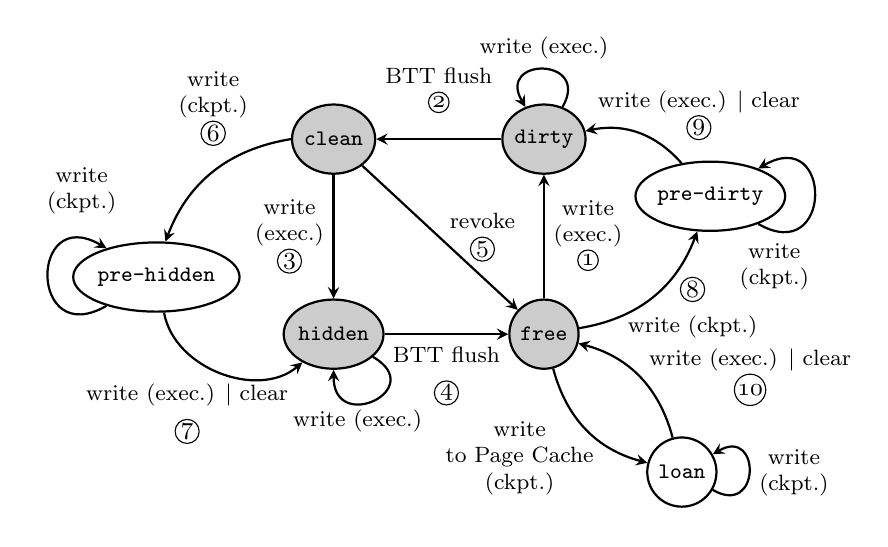
\begin{tikzpicture}[->, >=stealth, node distance=0.37\tikzdistance, auto, thick,
font=\footnotesize, text centered]

\tikzstyle{every state}=[ellipse, inner sep=0pt]

\node[state] (h) [fill={rgb:black,1;white,4}] {\state{hidden}};
\node[state] (f) [right=of h, fill={rgb:black,1;white,4}] {\state{free}};
\node[state] (c) [above=of h, fill={rgb:black,1;white,4}] {\state{clean}};
\node[state] (t) [below left=of c] {\state{pre-hidden}};
\node[state] (d) [above=of f, fill={rgb:black,1;white,4}] {\state{dirty}};
\node[state] (s) [above right=of f] {\state{pre-dirty}};
\node[state] (l) [below right=of f] {\state{loan}};

\path (c.west)
  edge [bend right, anchor=south]
    node {\makecell[c]{write\\(ckpt.)\\\circled{$\mathnormal{6}$}}} (t);
\path (c)
  edge [anchor=east] node {\makecell[c]{write\\(exec.)\\\circled{$\mathnormal{3}$}}} (h)
  edge [anchor=west] node {\makecell[c]{revoke\\\circled{$\mathnormal{5}$}}} (f);
\path (h)
  edge [anchor=north] node {\makecell[c]{BTT flush\\\circled{$\mathnormal{4}$}}} (f)
  edge [loop, out=330, in=270, anchor=north, looseness=4]
    node [xshift=-0.05\tikzdistance] {write (exec.)} (h);
\path (t)
  edge [bend right, out=300, in=240, anchor=north]
    node [xshift=-0.1\tikzdistance] {\makecell[c]{write (exec.) $|$ clear\\\circled{$\mathnormal{7}$}}} (h)
  edge [loop, out=210, in=150, looseness=4, anchor=south]
    node [xshift=0.1\tikzdistance, yshift=0.15\tikzdistance]
      {\makecell[c]{write\\(ckpt.)}} (t);
\path (f)
  edge [anchor=west] node {\makecell[c]{write\\(exec.)\\\circled{$\mathnormal{1}$}}} (d)
  edge [bend right, anchor=base]
    node [xshift=0.12\tikzdistance, yshift=-0.05\tikzdistance] {\makecell[c]{\circled{$\mathnormal{8}$}\\write (ckpt.)}} (s)
  edge [bend right, anchor=base]
    node [xshift=-0.2\tikzdistance, yshift=-0.1\tikzdistance] {\makecell[c]{write\\to \region{Page Cache}\\(ckpt.)}} (l);
\path (s)
  edge [bend right, anchor=west]
    node [xshift=-0.15\tikzdistance, yshift=0.05\tikzdistance]
      {\makecell[c]{write (exec.) $|$ clear\\\circled{$\mathnormal{9}$}}} (d)
  edge [loop, out=330, in=30, anchor=north, looseness=4]
    node [xshift=-0.12\tikzdistance, yshift=-0.1\tikzdistance]
      {\makecell[c]{write\\(ckpt.)}} (s);
\path (d)
  edge node [anchor=south] {\makecell[c]{BTT flush\\\circled{$\mathnormal{2}$}}} (c)
  edge [loop, out=60, in=120, looseness=4, anchor=south]
    node {write (exec.)} (d);
\path (l)
  edge [bend right, anchor=west]
    node {\makecell[c]{write (exec.) $|$ clear\\\circled{$\mathnormal{10}$}}} (f)
  edge [loop, out=330, in=30, looseness=4, anchor=north]
    node [anchor=west] {\makecell[c]{write\\(ckpt.)}} (l);

\end{tikzpicture}


\caption{在块重映射模式下,一个BTT表项的状态。每个内存写(“write”)后注明“exec.”或“ckpt.”,分别意味着该内存写到来的时间在程序执行阶段(无检查点生成)或在检查点生成阶段;“write'”指原本应到页缓存的写。}
\label{fig:thynvm-state-machine}
\end{figure}

\subsection{执行时的状态}

该组状态主要协调模式在程序执行(没有检查点生成)时的行为。为了决定内存写的正确地址,我们需要一个状态记录关于地址映射的两方面信息:(1)该物理地址在当前活跃时间单元内是否被写过。如果是的话,我们可以直接覆写对应的硬件地址,因为同一个时间单元内对相同物理地址的内存写可以合并。(2)硬件地址是一个主硬件地址还是位于检查点区域中。在某些情况下,如果我们需要避免覆写其中一个的话,我们将选择另外一个。据此,我们有四个状态来涵盖上述两个选择的所有组合。

\begin{itemize}
\item \textbf{\state{Free}态}:标志一个空的无有效映射的表项。同时我们将没有包含在BTT中的物理地址默认为\state{free}态。这意味着其物理地址在当前活跃时间单元内没有被更改过,且其检查点数据位于家区域中的主硬件地址。新来的对该物理地址的写请求必须在BTT中开辟一个新的表项将这个写重映射到块检查点区域。

\item \textbf{\state{Clean}态}:该状态表明其物理地址在当前活跃时间单元没有被更改过,且其检查点数据位于块检查点区域。新来的对该物理地址的写请求必须被BTT重映射到家区域的主硬件地址以保护检查点数据。

\item \textbf{\state{Dirty}态}:该状态表明其物理地址在当前活跃时间单元内被更改过,且对应的硬件地址在块检查点区域。该映射可以继续有效直到当前时间单元结束,用以合并到相同物理地址的内存写。在当前时间单元结束后,该硬件地址上的数据应当变为检查点数据,所以这个表项会被备份到NVM,将映射关系持久化,以备系统故障时定位检查点数据。

\item \textbf{\state{Hidden}态}:这个状态表明其物理地址在当前活跃时间单元内被更改过,且对应的硬件地址是位于家区域的主硬件地址。这里实际上并没有地址转换,因为主硬件地址和物理地址是相等的。然而,该表项会一直存在直到当前时间单元结束,目的是合并同时间单元内对该物理地址的其他写。在当前时间单元结束后,这个表项会被清除。
\end{itemize}

\vspace{\noindentsep}
\noindent \textbf{实例  }为了展示上述状态之间的动态转换,我们构造了图~\ref{fig-example}中的实例。我们首先忽略检查点生成期间的步骤(步骤A和B),并简单假设它们没有发生。在这个实例中,我们展示了三个连续的时间单元,记为时间单元0到2。从时间单元$k$收到的内存写会产生数据版本$v_k$,其中$k = 0, 1, 2$。

\begin{figure}[!ht]
\centering
\includegraphics[width=\linewidth]{figures/example.pdf}
\caption{连续时间单元中对物理地址P进行多次内存写的实例。}
\label{fig-example}
\end{figure}

\vspace{\noindentsep}
\noindent\ding{202} 初始状态,我们假设在物理地址P的数据位于其主硬件地址(家区域),所以在BTT中没有对应的表项,且不占用块检查点区域或块缓存区域的位置。P位置的数据可以认为是最近检查点的版本(标记为$v_{-1}$,即$v_0$之前的一个版本)。

\vspace{\noindentsep}
\noindent\ding{203} 在执行时间单元0的过程中,当一个对物理地址P的内存写到达时,我们不能覆写家区域中的检查点数据$v_{-1}$。所以,一个新的映射P-N被添加到BTT中,将数据$v_0$导向块检查点区域中的硬件地址N。我们将该表项标记为\state{dirty}态(图~\ref{fig:thynvm-state-machine}中的状态转换\circled{$\mathnormal{1}$})以表明该物理地址在当前活跃时间单元内已经被更改过。这个时间单元内后续的任意对物理地址P的内存写都可以合并在硬件地址N。

\vspace{\noindentsep}
\noindent\ding{204} 在时间单元0之后,上述\state{dirty}表项被冲刷到BTT/PTT/CPU备份区域。该表项在BTT中的状态变为\state{clean}(状态转换\circled{$\mathnormal{2}$})以表明该映射已经持久化且在新的时间单元1中尚无对该物理地址的写。

\vspace{\noindentsep}
\noindent\ding{205} 时间单元0完成检查点生成之后,我们不再需要家区域中的数据$v_{-1}$。所以对物理地址P的内存写可以直接映射到主硬件地址。与此同时,相应的BTT表项状态变为\state{hidden}态(状态转换\circled{$\mathnormal{3}$})。该状态表明主硬件地址保存着数据$v_1$,而且这个时间单元内对P的后续写可以在这个位置上更新数据。如果这一步出现系统故障,ThyNVM则会回退到块重映射区域保存的数据$v_{0}$。

\vspace{\noindentsep}
\noindent\ding{206} 当时间单元2开始时,BTT冲刷操作已经将\state{hidden}状态清除,而这个表项被释放以表明家区域中的主硬件地址保存着物理地址P的数据的最近检查点版本$v_1$(状态转换\circled{$\mathnormal{4}$})。

我们可以看到,该BTT表项在连续多个时间单元收到内存写之后会变为\state{free}态。所以,多个时间单元之间的时间局部性可以减少使用中的表项,进而缓解对有限的BTT的存储空间的压力。在最坏状态下,如果BTT没有\state{free}状态的表项,我们必须撤销一个\state{hidden}态或者\state{clean}态的表项为新的内存写提供空间。\state{Hidden}态的表项无论如何都会在当前活跃时间单元结束时被撤销;
\state{Clean}态的表项可以被安全撤销(状态转换\circled{$\mathnormal{5}$})是因为他们不记录当前活跃时间单元内的新的更新。然而,被\state{clean}态表项引用的数据块(位于块检查点区域)需要和其主硬件地址上的数据互换。

\subsection{检查点生成时的状态}
\label{subsec:states-ckpt}

第二个状态组在检查点生成阶段发挥作用。该组包含两个状态,\state{pre-hidden}态和\state{pre-dirty}态,分别处理如下两种情况。

\begin{itemize}
\item
\textbf{\state{Pre-hidden}}态:该状态处理一个\state{clean}态的物理地址在检查点生成阶段收到内存写的情况。我们不能简单地像程序执行阶段一样执行状态转换\circled{$\mathnormal{3}$},因为家区域和块检查点区域的数据在检查点生成阶段都必须被保留。以图~\ref{fig-example}中的步骤A为例。因为我们当前处于时间单元1,块检查点区域的数据$v_0$是不可更改的,因为它是最近检查点 \cl 的一部分;同样地,家区域中的数据$v_{-1}$也不可更改,因为完整的一致的 \cl 尚未完成——如果此时系统故障终断了检查点生成进程,系统会回滚到$v_{-1}$(即 \cp)。因此,我们需要临时将工作数据(\wa)放入另外一个地方,块缓存区域,并相应地把这个特别的状态标记为\state{pre-hidden}(状态转换\circled{$\mathnormal{6}$})。\state{Pre-hidden}状态是\state{clean}状态和\state{hidden}状态之间的一个垫脚石。它只在当前活跃时间单元结束前存在。之后,如果该状态没有被一个内存写驱动转换到\state{hidden}(达到图~\ref{fig-example}中步骤4相同的结果),它会被显式地清理(状态转换\circled{$\mathnormal{7}$})。不论哪种情况,因为时间单元0的检查点(\cl)已经完成,版本$v_{-1}$(\cp)都会被工作数据 \wa 安全地覆写,并相应收回块缓存区域里 \wa 的位置。
\item
\textbf{\state{Pre-dirty}}态:该状态处理一个\state{free}态的物理地址在检查点生成阶段收到内存写的情况。与\state{pre-hidden}的处理逻辑类似,我们不能像程序执行阶段一样直接执行状态转换\circled{$\mathnormal{1}$}。以图~\ref{fig-example}中的步骤B为例。当时间单元1的检查点(\cl)正在生成的时候,我们不仅要保留$v_1$,还要保留$v_0$(\cp),因为 \cp 是我们仅有的完整一致的检查点。所以,我们把数据$v_2$放入块缓存区域,并向BTT添加一个\state{pre-dirty}态的表项来记录该映射(状态转换\circled{$\mathnormal{8}$})。\state{Pre-dirty}状态或者被下一个程序执行阶段的内存写命中转换到\state{dirty}态,或者在那个阶段结束时被清理转换到\state{dirty}态(状态转换\circled{$\mathnormal{9}$})。
\end{itemize}

因为\state{hidden}态和\state{dirty}态在每个检查点生成阶段刚刚开始时伴随BTT冲刷操作被清理,他们永远不会在检查点生成阶段与内存写相遇。所以,我们没有其他情况需要处理。

\subsection{用于双模式合作的状态}

最后我们有一个用于两个模式间合作的状态。当页回写模式生成脏页的检查点时,对这些页的各个内存写暂由块重映射模式重定向到块缓存区域(与第\ref{subsec:states-ckpt}节介绍的操作类似)。我们不把这些BTT表项混入上文的那些状态和转换,所以这些表项被标记为\state{loan}。当检查点生成结束这些页面重新可以被直接修改的时候,\state{Loan}态的表项最终将数据移回原页中(状态转换\circled{$\mathnormal{10}$})。

\section{正确性定义}

本节给出一致性协议正确性证明的定义。我们这里聚焦于ThyNVM检查点生成模式的故障时一致性,亦即可恢复性——任何时候系统发生故障,ThyNVM可以恢复最近的一致的检查点。特别地,假设$t_k$为时间单元$k$结束执行的时刻,那么在$t_{k-1}$和$t_k$之间,ThyNVM顺次经历两个时间阶段,即一个检查点生成阶段(与时间单元$k+1$的程序执行阶段重合)和一个程序执行阶段(指没有与检查点生成重合的部分);$t_k$时刻的数据快照记为版本$v_k$,亦即时间单元$k$的检查点版本。我们将证明如下两个不变式,在状态机的转换中一直保持成立。

\begin{enumerate}
\item \label{invar-ckpt} 在时刻$t_{k-1}$与$t_k$之间的检查点生成阶段,数据版本$v_{k-1}$和$v_{k-2}$及其在地址转换表中的映射都被保留。
\item \label{invar-exec} 在时刻$t_{k-1}$与$t_k$之间的程序执行阶段,数据版本$v_{k-1}$及其在地址转换表中的映射都被保留。
\end{enumerate}

显然,如果上述两个不变式成立,那么系统在检查点生成阶段或程序执行阶段发生故障时,可以分别恢复到{\cp}或{\cl}。

\section{块重映射模式的正确性证明}

ThyNVM的块重映射模式由第\ref{subsec:thynvm-state-machin}节的状态机描述。对于任何由状态机转换形成的状态序列,我们使用数学归纳法\cite{Hopcroft:ALC:2006}验证上节两个不变式的正确性。

\subsection{数据抽象}

为了实施形式化证明,我们使用变量来代表ThyNVM中的数据结构,如图\ref{fig-data-struct}所示。由于我们只关心数据版本而非具体的数据,不妨认为这些变量保存着数据版本值;大写的变量值表示集合。因为所有 BTT表项互斥,我们仅关心任意一个BTT表项,并假设该表项当前是用于物理地址\phy{P}。

\begin{figure}[!t]
\centering
\includegraphics[width=0.9\columnwidth]{data-struct}
\caption{ThyNVM中的数据结构及其符号。}
\label{fig-data-struct}
\end{figure}

\begin{itemize}
\item $p$ 保存着主硬件地址\nvm{P}上的数据块的版本号。
\item $T$ 保存着对应于\phy{P}的BTT表项。该表项是易失的。如果没有对应于\phy{P}的BTT表项,那么
$T=\varnothing$,此时可认为\phy{P}的状态为\state{free};否则,我们恒有$\left\vert{T}\right\vert = 1$,其中唯一的项保存着在块检查点区域中对应数据块的版本号。
\item $T^B$ 保存着持久化的BTT表项,位于BTT备份区域。类似地,我们有$\left\vert{T^B}\right\vert \le 1$。特别地,对于时间单元$0$,我们仅出于方便计算的目的认为$T^B \subset \{-1, -2\}$。
\end{itemize}

另外,下面的字母代BTT表项状态机的输入。

\begin{itemize}
\item $\mathbf{w}$和$\mathbf{\hat{w}}$分别表示在程序执行阶段和检查点生成阶段向物理地址\phy{P}的写操作。
\item $\mathbf{r}$和$\mathbf{\hat{r}}$分别表示在程序执行阶段和检查点生成阶段撤销物理地址\phy{P}对应的BTT表项。
\item $\mathbf{f}$表示刷出BTT到备份区域。该事件标志一个检查点阶段的开始。
\item $\mathbf{c}$表示在刷出BTT之前清理\state{pre-dirty}态和\state{pre-dirty}态表项的操作。
\end{itemize}

\subsection{行为抽象}

基于如上的变量和符号,我们将主要的状态转换过程表述为过程\ref{alg-dirty}到\ref{alg-free-c}。相应地,BTT表项的状态机也可改写为图\ref{fig:asm}。注意\state{loan}态没有在图中画出,而是在第\ref{sec:proof-page-writeback}节单独讨论。

\begin{algorithm} [!h]
\caption{转换至\state{dirty}态}
\label{alg-dirty}
\begin{algorithmic}[1]
\Require 处于程序执行阶段。
\State 在块检查点区域分配地址\nvm{N}
\State 将数据块$v_0$写入\nvm{N}
\If{表项是\state{pre-dirty}态,即映射关系为\phy{P}-\dram{D}}
  \State 从块缓存区域撤销位于\dram{D}的数据块
\EndIf
\State 设置表项为\state{dirty}态,即映射关系为\phy{P}-\nvm{N} \Comment{$T \leftarrow \{0\}$}
\end{algorithmic}
\end{algorithm}

\begin{algorithm} [!h]
\caption{临时缓存数据块}
\label{alg-hold}
\begin{algorithmic}[1]
\Require 处于检查点生成阶段。
\State 在块缓存区域分配地址\dram{D}
\State 将数据块$v_0$写入\dram{D}
\If{表项是\state{clean}态,即映射关系为\phy{P}-\nvm{N}}
  \State 将位于\nvm{N}的数据标记为在下一个检查点生成阶段被撤销
  \State 将表项转换至\state{pre-hidden}态
\ElsIf{表项是\state{free}态}
  \State 将表项转换至\state{pre-dirty}态
\EndIf
\State 设置映射关系为\phy{P}-\dram{D} \Comment{$T \leftarrow \{0\}$}
\end{algorithmic}
\end{algorithm}

\begin{algorithm} [!h]
\caption{转换至\state{hidden}态}
\label{alg-hide}
\begin{algorithmic}[1]
\Require 处于程序执行阶段。
\State 将数据块$v_0$写入主硬件地址 \Comment{$p \leftarrow 0$}
\If{表项是\state{clean}态,即映射关系为\phy{P}-\nvm{N}}
  \State 将位于\nvm{N}的数据标记为在下一个检查点生成阶段被撤销
\ElsIf{表项是\state{pre-hidden}态,即映射关系为\phy{P}-\dram{D}}
  \State 从块缓存区域撤销位于\dram{D}的数据块
\EndIf
\State 将表项转换至\state{hidden}态 \Comment{$T \leftarrow \{p\}$}
\end{algorithmic}
\end{algorithm}

\begin{algorithm} [!h]
\caption{撤销\state{clean}态的映射关系\phy{P}-\nvm{N}}
\label{alg-free-c}
\begin{algorithmic}[1]
\If{处于程序执行阶段}
  \State 将位于\nvm{N}的数据块$v_{-1}$写入\nvm{P},覆盖数据块$v_{-2}$ \Comment{$p \leftarrow -1$}
  \State 将位于\nvm{N}的数据标记为在下一个检查点生成阶段被撤销
\Else \Comment{处于检查点生成阶段}
  \State 交换位于\nvm{P}的数据块$v_{-2}$和位于\nvm{N}的数据块$v_{-1}$ \Comment{$T^B \leftarrow (T^B - T) \cup \{p\}$}
  \Statex \Comment{$p \leftarrow -1$}
  \State 在BTT备份(对应于$v_{-1}$)中标记\phy{P}-\nvm{N}为已置换
  \State 将位于\nvm{N}的数据块标记为在下一个检查点生成阶段被撤销
\EndIf
\State 将表项转换至\state{free}态,即撤销该表项 \Comment{$T \leftarrow \{p\}$}
\end{algorithmic}
\end{algorithm}

\begin{figure}[!t]
\centering
\begin{tikzpicture}[->, >=stealth, node distance=0.38\tikzdistance, auto, thick,
font=\footnotesize]

\tikzstyle{every state}=[ellipse, inner sep=1pt]

\node[state] (h) {\state{hidden}};
\node[state] (f) [right=of h] {\state{free}};
\node[state] (c) [above=of h] {\state{clean}};
\node[state] (t) [below left=of c] {\state{pre-hidden}};
\node[state] (d) [above=of f] {\state{dirty}};
\node[state] (s) [above right=of f] {\state{pre-dirty}};

\path (c.west)
  edge [bend right, anchor=south]
    node [xshift=-0.18\tikzdistance]
      {\trans{\mathbf{\hat{w}}}{Procedure~\ref{alg-hold}}} (t);
\path (c)
  edge [bend right, anchor=base]
    node {\trans{\mathbf{w}}{Procedure~\ref{alg-hide}}} (h)
  edge [anchor=base] node {\trans{\mathbf{r, \hat{r}}}{Procedure~\ref{alg-free-c}}} (f);
\path (h)
  edge [anchor=south] node {$\mathbf{f}$} (f)
  edge [loop, out=330, in=270, anchor=north, looseness=4]
    node {$\mathbf{w}$} (h);
\path (t)
  edge [bend right, out=300, in=240, anchor=north]
    node {\trans{\mathbf{w, c}}{Procedure~\ref{alg-hide}}} (h)
  edge [loop, out=210, in=150, looseness=4, anchor=south]
    node [xshift=0.1\tikzdistance, yshift=0.15\tikzdistance]
      {$\mathbf{\hat{w}}$} (t);
\path (f)
  edge [bend right, anchor=base]
    node {\trans{\mathbf{w}}{Procedure~\ref{alg-dirty}}} (d)
  edge [bend right, anchor=west]
    node {\trans{\mathbf{\hat{w}}}{Procedure~\ref{alg-hold}}} (s);
\path (s)
  edge [bend right, anchor=south]
    node [xshift=0.15\tikzdistance]
      {\trans{\mathbf{w, c}}{Procedure~\ref{alg-dirty}}} (d)
  edge [loop, out=330, in=30, anchor=south, looseness=4]
    node [xshift=-0.12\tikzdistance, yshift=0.15\tikzdistance]
      {$\mathbf{\hat{w}}$} (s);
\path (d)
  edge node [anchor=south] {$\mathbf{f}$} (c)
  edge [loop, out=60, in=120, looseness=4, anchor=south]
    node {$\mathbf{w}$} (d);

\end{tikzpicture}


\caption{BTT表项的状态机的抽象描述,用于实现块重映射模式。}
\label{fig:asm}
\end{figure}

\subsection{证明步骤}

每一个输入的写操作驱动状态机进行一步转换。 因此,我们可以为所有变量添加一个下标$n$,以标示变量值对应于状态机状态转换序列中的哪一步。我们采用数学归纳法的证明基于$n$进行推导。

\textbf{命题}:不变式~\ref{invar-exec}和不变式~\ref{invar-ckpt}可以分别翻译为如下两个命题$P(n)$和$Q(n)$。

在程序执行阶段,我们需要保证$P(n)$一直成立:$$ P(n)=(-1 \in T^B_n) \vee (-1 \notin T^B_n \wedge p_n=-1). $$ 我们假设当前活跃时间单元为0。上式隐含了两个可以接受的情况。第一个是BTT备份包含一个指向块检查点区域的映射(即$-1 \in T^B_n$)。第二个是BTT备份不包含对$v_{-1}$的映射关系(即$-1 \notin T^B_n$)但{\cl}处于主硬件地址(即$p_n=-1$)。只要两个情况任一成立,那么系统故障发生时,从BTT备份中恢复出BTT可使ThyNVM找到地址\phy{P}的正确的{\cl},即$v_{-1}$。

在检查点生成阶段,我们需要保证$Q(n)$一直成立:$$ Q(n)=(p_n=-2 \wedge -1 \in T^B_n) \vee (p_n=-1 \wedge -2 \in T^B_n). $$ 与$P(n)$类似,$Q(n)$意味着两个正确的情况:BTT备份包含{\cl}($v_{-1}$)的映射并指向块检查点区域(即$-1 \in T^B_n$),而\cp($v_{-2}$)位于主硬件地址,依然得到保留(即$p_n=-2$);或者两个版本所处位置相反的情况——如果主硬件地址保存着{\cl},那么BTT备份必须记录着{\cp}的位置(即$p_n=-1 \wedge -2 \in T^B_n$)。

综上,我们需要证明如下这个命题:$$S(n)=(\alpha_n \in
\{\mathbf{w}, \mathbf{r}, \mathbf{c}\} \wedge P(n)) \vee (\alpha_n \in
\{\mathbf{\hat{w}}, \mathbf{\hat{r}}, \mathbf{f}\} \wedge Q(n))$$
我们通过区分输入的字母$\alpha_n$来判断处于程序执行阶段还是检查点生成阶段。 $\mathbf{w}、\mathbf{r}$和$\mathbf{c}$在程序执行阶段输入,而其余的在检查点生成阶段出现。

\textbf{归纳基础}:
在整个系统最初始的状态,我们可以认为所有数据均位于主硬件地址。不妨假设初始步骤前存在虚拟的时间单元-1,那么有$p_0=-1$;另外,由于BTT为空,我们有$T^B_0=\varnothing$。所以,$P(0)$成立。进而,由于处在程序执行阶段,$S(0)$是成立的,值为真。

\noindent\textbf{归纳步骤}:
假设对任意的$n \ge 1$,$S(n-1)$为真,下面我们论证$S(n)$也为真。

首先,我们统一考虑状态机中所有自循环。对于状态\state{dirty}、\state{pre-dirty}和\state{pre-hidden},ThyNVM只更新$T_n$,所以$S_n=S_{n-1}$为真。对于状态\state{hidden},ThyNVM令$p_n=0$,但根据将状态转换至\state{hidden}的过程\ref{alg-hide},在自循环前即有$p_{n-1}=0$,所以ThyNVM并没有更改该值。所以我们也可以得到$S_n=S_{n-1}$。

其次,我们看两个包含BTT冲刷$\mathbf{f}$的状态转换。

$\state{dirty} \rightarrow \state{clean}$:转换前的状态为\state{dirty}表明$p_{n-1}=-1$。转换后,新的时间单元与检查点生成阶段重合,所以我们有$p_n=-2$\footnote{只有BTT刷出操作会将所有的版本号减一。任何其他过程中,版本号或者保持或者被显式赋值}。另外,ThyNVM将\state{clean}态的映射写入BTT备份,意味着$-1$被加入$T^B_n$。所以,我们有$p_n=-2 \wedge -1 \in T^B_n$,也就是$Q(n)$成立。进而,$S(n)$为真。

$\state{hidden} \rightarrow \state{free}$:转换前的状态是\state{hidden}意味着$p_{n-1}=0$,而在程序执行阶段,$S(n-1) \implies P(n-1)$,所以$-1 \in T^B_{n-1}$必为真。状态转换之后,由于处在新的时间单元,我们有$p_n=-1$以及$-2 \in T^B_n$。所以$Q(n)$为真,进而$S(n)$成立。

除去上述情况,步骤$n$必然经历下面的过程。

过程\ref{alg-dirty}管理着状态转换$\state{free} \rightarrow
\state{dirty}$和$\state{pre-dirty} \rightarrow \state{dirty}$。不论哪个状态转换,该过程保护$p=-1 \wedge -1 \notin T^B$:转换前,状态\state{free}和\state{pre-dirty}都有$p_{n-1}=-1 \wedge -1 \notin
T^B_{n-1}$,而该过程避免覆写主硬件地址,所以我们有$p_n=-1$。而且,该过程不刷出表项到BTT备份区域,所以有$-1 \notin T^B_n$。因此,$P(n)$成立。又因为处在程序执行阶段(即$\alpha_n \in \{\mathbf{w}, \mathbf{r}, \mathbf{c}\}$),我们有$S(n-1) \implies S(n)$。

过程\ref{alg-hold}管理着状态转换$\state{clean} \rightarrow
\state{pre-hidden}$和$\state{free} \rightarrow \state{pre-dirty}$。不论哪个状态转换,该过程将数据写入块缓存区域,而不是更改$p$或$T^B$。这么做的目的是在检查点生成阶段保护$v_{-1}$和$v_{-2}$。因此,不难得出$S(n)=S(n-1)$。

过程\ref{alg-hide}管理着状态转换$\state{clean} \rightarrow
\state{hidden}$和$\state{pre-hidden} \rightarrow \state{hidden}$。转换前,状态\state{clean} 和\state{pre-hidden}必然处在检查点生成阶段,所以有$p_{n-1}=-2 \wedge -1 \in T^B_{n-1}$ (根据BTT刷出行为和过程\ref{alg-hold})。在该过程中,ThyNVM设置$p_n=0$但不涉及$T^B$,所以我们有$p_n=0 \wedge -1 \in T^B_n$。又因为处于程序执行阶段,$S(n)$为真。

过程\ref{alg-free-c}管理着状态转换$\state{clean} \rightarrow \state{free}$,但有可能处于程序执行阶段,也可能处于检查点生成阶段。状态转换器前,依据BTT刷出行为我们有
$P_{n-1}=-2 \wedge -1 \in T^B_{n-1}$,且被$T$引用的最近的版本是$v_{-1}$。如果处于程序执行阶段,该过程设置
$p_n=-1$,但保持$-1 \in T^B_n$,所以$P(n)$成立。进而,$S(n)$为真。如果处于检查点生成阶段,ThyNVM交换$p$和$T^B$的值,从而导致
$p_n=-1 \wedge -2 \in T^B_n$。相应地,$Q(n)$成立,且$S(n)$为真。

综上,对于状态机在所有可能的转换中所遵循的路径,恒有$S(n-1)
\implies S(n)$。考虑到初始步骤0符合$S(0)$,我们可以得出结论$S(n)$对所有的$n \ge 0$成立。也就是说,不变式\ref{invar-ckpt}和\ref{invar-exec}对任何物理地址均成立。


%Finally, we explain why the number of \textsc{Block Buffer} slots should be twice
%the number of BTT entries, even though any particular physical address only
%requires up to one slot in \textsc{Block Buffer} as shown above. Apparently, we
%have $\left\vert{T^B}\right\vert \le 1$ for any single physical address served
%by BTT, and it references up to one \textsc{Block Buffer} slot. However, when
%there is a \state{free} BTT entry, it may serve a different physical address
%upon request. This does not affect consistency or recoverability of either
%address, but requires extra \textsc{Block Buffer} slots as the new address may
%need a second \textsc{Block Buffer} slot. For example, suppose a BTT entry for
%\phy{P} shifts from \state{clean} to \state{free} in an execution phase, then we
%have $-1 \in T^B$ and it references a \textsc{Block Buffer} slot. Afterwards, if we
%receive a write to another physical address \phy{P'}, we may have to set up a
%\state{dirty} mapping for \phy{P'} using this \state{free} entry. In that case, $T$ maps
%to a second slot in \textsc{Block Buffer}.
%
%Meanwhile, no matter how many physical addresses the BTT serves, we have at most
%two versions of full BTT in \textsc{BTT Backup}, so they reference \textsc{Block
%Buffer} slots of at most twice the number of BTT entries. Further, when
%\textsc{Block Buffer} slots are occupied by previous versions of data ($v_{-1}$
%and $v_{-2}$ referenced by \textsc{BTT Backup}), the current version of data
%($v_0$) will locate in \textsc{Block Cache} via \state{pre-hidden} and
%\state{pre-dirty}.

\section{页回写模式的正确性证明}
\label{sec:proof-page-writeback}

为了简便,我们在证明中忽略不重要的部分。首先,我们认为如下\emph{独立的回写模式}的正确性自明:(1)在检查点生成阶段停止一切对内存的修改;(2)将缓存的脏页写入NVM作为检查点,但是不覆写它们之前的版本;(3)原子性地将记录所有检查点页位置的表写入NVM。显然,不变式\ref{invar-ckpt}和\ref{invar-exec}都是成立的。 

对于上述步骤(2),我们重用块重映射模式的状态机来维护故障时数据一致性。特别地,我们只需做如下替换:第一,块重映射协议中的程序执行阶段和检查点生成阶段在这个过程中都被认为是程序执行阶段,所以只有\state{free}、
\state{dirty}、\state{clean}和\state{hidden}四个状态有效。第二,块检查点区域由页检查点区域代替。第三,所有写变为页粒度,而不再是块粒度。因此,这个过程可以视作之前论证的重映射模式的一个特例,其正确性可以得到保证。

进而,基于上述独立的回写模式的正确性,我们可以得出ThyNVM采用的页回写模式的正确性。当生成脏页的检查点时,块重映射模式会临时负责代理应用程序写往页缓存区域的新的请求,所以ThyNVM的页回写模式与独立的页回写模式等价,当且仅当满足如下两个条件:(1)页缓存区域保存着在生成检查点开始前保存着数据的最新的一致的版本;(2)页缓存区域的这一状态在整个检查点生成阶段得以保持。

第一个条件可以满足,因为在程序执行阶段页缓存区域是直接更新的,而保存在块缓存区域中的数据会在检查点生成阶段前移回页缓存区域(由一个清理操作完成)。第二个条件也成立,因为在检查点生成阶段,应用程序的新的写都被转移到块缓存区域而不会污染页缓存区域。综上,ThyNVM的页回写模式被证明是正确的。

\chapter{总结与展望}
\label{chap:conclusion}

\section{工作总结}

持久性内存系统可能对当前计算机体系结构产生重大影响。对于使用持久性内存系统的最佳接口方式,学术界和产业界都在积极地探讨,尚未得出统一的结论。而影响这一选择的最主要因素就是故障时数据一致性的机制设计及其性能开销。为此,我在博士研究期间,从三种最主要的访问接口入手,系统地研究了持久性内存中高效的故障时数据一致性保证机制:(1)对于文件系统接口,现有研究较为充分,本文定位在更好地利用手机移动环境的特定属性上。我们的工作不需要特殊的硬件改动,即可支持持久性内存的系统假设,通过多版本缓存事务和新的优化策略,显著提高了应用的响应度和系统的能量效率。(2)对于事务性内存接口,本文定位在提升当前工作的可扩展性,使该类持久性内存可应用于大容量的闪存存储。为此,我们采用了快照隔离对只读负载隐藏持久化开销,并设计了小缓冲区组技术,可同时实现事务的高吞吐和低延迟。(3)对于软件透明的接口,本文定位在高效的硬件设计,通过新的双模式检查点技术,高效地实现内存控制器对故障时数据一致性的支持。此外,我们还给出了软件透明的一致性协议的状态机表述和形式化证明。

\section{未来展望}

基于本文的工作,非易失性内存硬件可以在系统结构的不同层面、在不同的应用场景下发挥积极作用。将非易失性内存用在文件系统中,可以更加灵活地选择数据刷出到二级存储的时间,获得更好的整体性能;将非易失性存储应用在事务性内存中,可以降低持久化的延迟和对事务吞吐的负面影响;对软件透明的基于硬件实现的持久化机制,可以使应用开发人员更加方便地利用内存持久化的优势,并且可以提升上层软件的兼容性和可移植性。我们相信,本文研究工作将推动持久性内存系统的实际应用。

与此同时,持久性内存系统,特别是其故障时数据一致性保证机制,对软硬件协同设计有较高的要求。本文部分工作还可以继续扩展和优化,以达到更好的性能指标。特别地,对软件透明的故障时数据一致性机制对内存数据状态的保证与传统事务性软件有所不同。上层应用在系统故障恢复后可以从\emph{适度滞后}但是一致的内存状态继续执行,却会面临设备错误以及和其他分布式系统结点间的同步问题。这些软件系统层面的挑战可能驱动上层系统设计和实现的改变,以更好地挖掘持久性内存的潜力和价值。



%%% 其它部分
\backmatter

% 本科生要这几个索引,研究生不要。选择性留下。
\makeatletter
\ifthu@bachelor
  % 插图索引
  \listoffigures
  % 表格索引
  \listoftables
  % 公式索引
  %\listofequations
\fi
\makeatother


% 参考文献
% 注意至少需要引用一篇参考文献,否则下面两行可能引起编译错误。
% 如果不需要参考文献,请将下面两行删除或注释掉。
\bibliographystyle{thubib}
\bibliography{ref/refs}


% 致谢
%%% Local Variables:
%%% mode: latex
%%% TeX-master: "../main"
%%% End:

% 如果使用声明扫描页,将可选参数指定为扫描后的 PDF 文件名,例如:
%\begin{ack}[scan-statement.pdf]
\begin{ack}

衷心感谢导师郑纬民教授和武永卫教授。他们在学术上悉心指导,在生活上关心照顾,为学生的发展构建了广阔的平台。忘不了和老师们的一次次讨论,忘不了老师们的谆谆教诲,也忘不了武老师在我的婚礼上作为主婚人的温馨致辞。

我还要感谢以往论文的其他合作者和指导者,他们的智慧亦融合在我的毕业论文中。微软亚洲研究院的Thomas Moscibroda和Mike Liang研究员为MobiFS项目的策略设计给予了宝贵建议。卡內基·梅隆大学(Carnegie Mellon University)的Onur Mutlu教授帮助我挖掘想法中价值,和时任惠普实验室(HP Labs)研究员的Jishen Zhao博士、时任英特尔研实验室(Intel Labs)研究员的Samira Khan博士一起反复修改我的论文。斯坦福大学(Stanford University)的David Cheriton教授和Heiner Litz博士多次斧正我的想法,他们组的工作为我的论文提供了很好的基础。我合作的论文中,当时威斯康星大学麦迪逊分校(University of Wisconsin–Madison)的Shan Lu教授给予的帮助和指导,在此一并感谢;原SanDisk副总裁John Butsh博士、Facebook工程师Justin Meza博士对论文工作的判断和帮助也令我受益匪浅。此外,特别感谢清华实验室的陈康老师、蒋进磊老师、黄小猛老师、杨广文老师等多年来寄予的指导和照顾;师兄弟刘立坤、张扬、祝美祺、章明星、王博、郭维超、赵勋、牟帅、王秋平、叶丰、苏茂萌、高品等同学,不断和我分享着他们的创见、努力和一起玩乐的美好时光。

感谢我的妻子闫睿颖女士,她无私无畏的支持和先于我工作所给予的经济援助,帮我度过了无数难关。儿子任念初的到来,赐予我生命的灵感和前行的动力。更要感谢我的父母任东兴、任焕茹,我的岳父母闫子政、张世平,他们构筑了我多年科研工作的坚实后方,是我毕业论文能够成文的不可磨灭的功臣。

最后,感谢自然科学基金、国家863计划、国家973计划、龙门教育基金、登峰基金、斯坦福大学计算机科学系等对本人工作的资助。感谢答辩委员会专家及匿名评审专家的宝贵时间和指导。

\end{ack}


% 附录
%\begin{appendix}
%\input{data/appendix01}
%\end{appendix}

% 个人简历
\begin{resume}

  \resumeitem{个人简历}

  1986 年 9 月 12 日出生于河北省保定市。

  2006 年 9 月考入东北师范大学软件学院软件工程专业,2010 年 7 月本科毕业并获得工学学士学位。

  2010 年 9 月免试进入清华大学计算机科学与技术系攻读硕士学位;2013 年 7 月转为提前攻读博士学位至今。

  博士在读期间,2013 年 11 月至 2014 年 5 月在卡内基梅隆大学(Carnegie Mellon University)做访问学者;2014 年 10 月至 2015 年 8 月在斯坦福大学(Stanford University)做访问研究员。

  \researchitem{发表的学术论文} % 发表的和录用的合在一起
% 学位论文写作指南:
% 在学期间发表的学术论文分以下三部分按顺序分别列出,每部分之间空 1
% 行,序号可连续排列
% 1. 已经刊载的学术论文(本人是第一作者,或者导师为第一作者本人是第二作者)
% 2. 尚未刊载,但已经接到正式录用函的学术论文(本人为第一作者,或者
% 导师为第一作者本人是第二作者)。
% 3. 其他学术论文。可列出除上述两种情况以外的其他学术论文,但必须是
% 已经刊载或者收到正式录用函的论文。
  \begin{publications}
  \item \textbf{Jinglei Ren}, Jishen Zhao, Samira Khan, Jongmoo Choi, Yongwei Wu, and Onur Mutlu.
Cooperative Checkpointing: A Software-Transparent Mechanism for Supporting Crash Consistency in Persistent Memory Systems, 
Proceedings of the 48th Annual IEEE/ACM International Symposium on Microarchitecture (MICRO), Dec. 2015.(CCF 推荐 A 类会议)
  \item \textbf{Jinglei Ren}, Chieh-Jan Mike Liang, Yongwei Wu, and Thomas Moscibroda.
Memory-Centric Data Storage for Mobile Systems, 
Proceedings of the 2015 USENIX Annual Technical Conference (USENIX ATC), Jul. 2015.(CCF 推荐 B 类会议)
  \item Mingxing Zhang, Yongwei Wu, Shan Lu, Shanxiang Qi, \textbf{Jinglei Ren}, and Weimin Zheng.
AI: A Lightweight System for Tolerating Concurrency Bugs 
Proceedings of the 22nd ACM SIGSOFT International Symposium on the Foundations of Software Engineering (FSE), Nov. 2014.(CCF 推荐 A 类会议)
  \item \textbf{Jinglei Ren}, Yongwei Wu, Meiqi Zhu, and Weimin Zheng.
Quatrain: Accelerating Data Aggregation Between Multiple Layers,
IEEE Transactions on Computers (TC), Vol. 63, No. 5, pp. 1207 - 1219, May 2014. (CCF 推荐 A 类期刊,SCI 检索)
  \item Yongwei Wu, Weichao Guo, \textbf{Jinglei Ren}, Xun Zhao, and Weiming Zheng.
NO2: Speeding Up Parallel Processing of Massive Compute-Intensive Tasks,
IEEE Transactions on Computers (TC), Vol. 63, No. 10, pp. 2487 - 2499, Oct. 2014.(CCF 推荐 A 类期刊,SCI 检索)
  \end{publications}

  \researchitem{研究成果} % 有就写,没有就删除
  \begin{achievements}
  \item 武永卫,任晶磊. : 中国, CNxxx. (中国专利公开号.)
  \item J. Ren, T. Moscibroda, M. Liang. : USA, No.xx/xxx, xxx. (美国发明专利申请号.)
  \end{achievements}
\end{resume}

\end{document}

